\documentclass[10pt,a4paper]{article}
\usepackage[utf8]{inputenc}
\usepackage{geometry}
\usepackage{float}
\usepackage{subfig}
\usepackage{graphicx}
\usepackage{caption}
\usepackage{booktabs} % To thicken table lines
\usepackage{diagbox}
\graphicspath{{q1_figs/}{q2a_figs/}{q2b_figs/}}
\title{CS6910 Assignment 1}
\author{Lakshya J(EE19B035), Neham Jain(EE19B084), Nisharg Manvar(EE19B094)}
\date{March 2022}

\begin{document}

\maketitle

\section{Function Approximation Task}
In this task, we are asked to create a Multi Layer Feed Forward Neural Network of two layers where the Learning Rate and the number of neurons in each layer are hyper-parameters.\\
\\
We are supposed to use Stochastic Gradient Descent as the optimizer and Mean Squared Error Loss for the loss function.\\
$tanh$ was used as the activation function after every layer except for the last output layer.\\
\\
I ran the model for 2000 epochs on  batch sizes of 16, 32, 64, 128 for varying learning rates and number of neurons.\\
\\
Learning rates used: [1e-6, 1e-5, 1e-4, 1e-3, 1e-2]\\
Number of neurons: [50, 100, 256, 512, 784, 1024, 2048]\\
\\
Out of all these cases, I observed the least loss for the validation set in the case of batch size of 16, learning rate = 0.01 and number of neurons = 512.\\
\\
Here is the result obtained:\\
$Learning\ Rate:\ 0.01\\
No.\ of\ Neurons:\ 50\\
Validation\ loss:\ 0.0003136$\\
\\
I tested this model on the test set to obtain final results.
\\
\newpage
\subsection{Plots Obtained}
First, I plot the 3D plot of the actual function.
\begin{figure}[htbp]
    \centering
    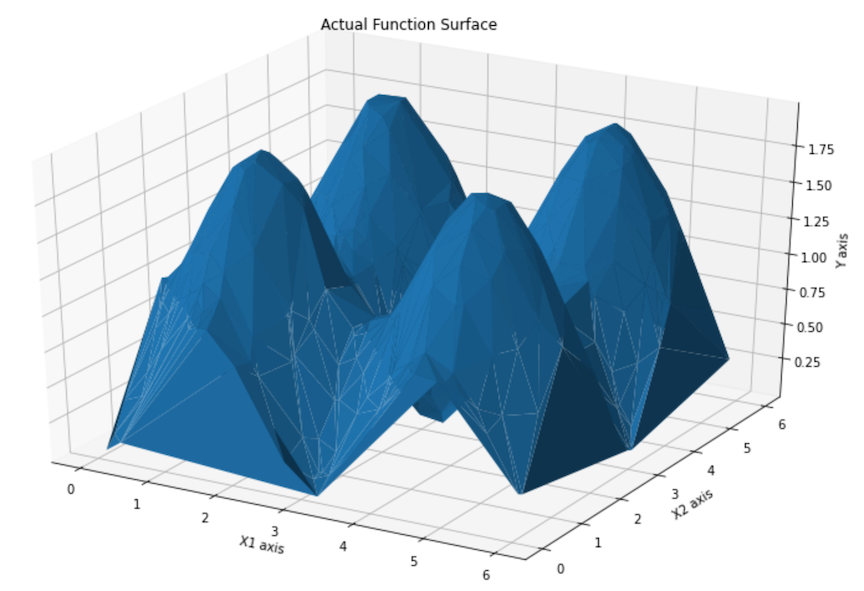
\includegraphics[width=0.8\linewidth]{ActualFunc.png}
    \captionsetup{justification=centering}
    \caption{Actual Plot}
\end{figure}
\\Next I plot the output obtained after training the model for various epochs. I plot the output of the model for epochs 1, 2, 10, 50, 500, 1000, 1500 and 2000(when the training is stopped).\\
It is observed that as the model moves through epochs, it is able to approximate the output better and give a smoother 3D output.
\begin{figure}[htbp]
    \centering
    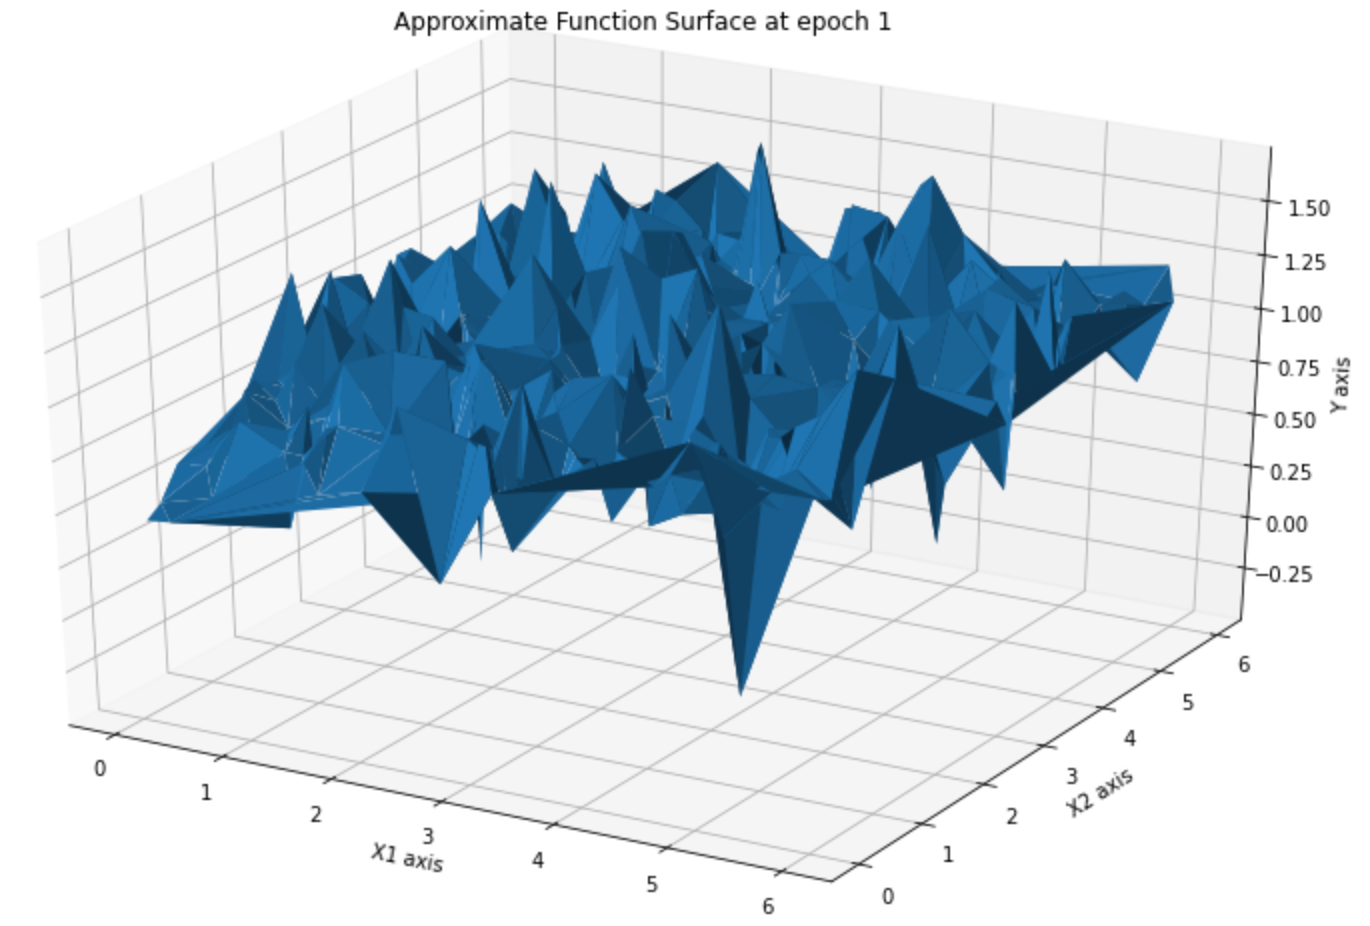
\includegraphics[width=0.8\linewidth]{Ep1.png}
    \captionsetup{justification=centering}
    \caption{Plot of all data applied on the model after 1 epoch}
\end{figure}
\begin{figure}[htbp]
    \centering
    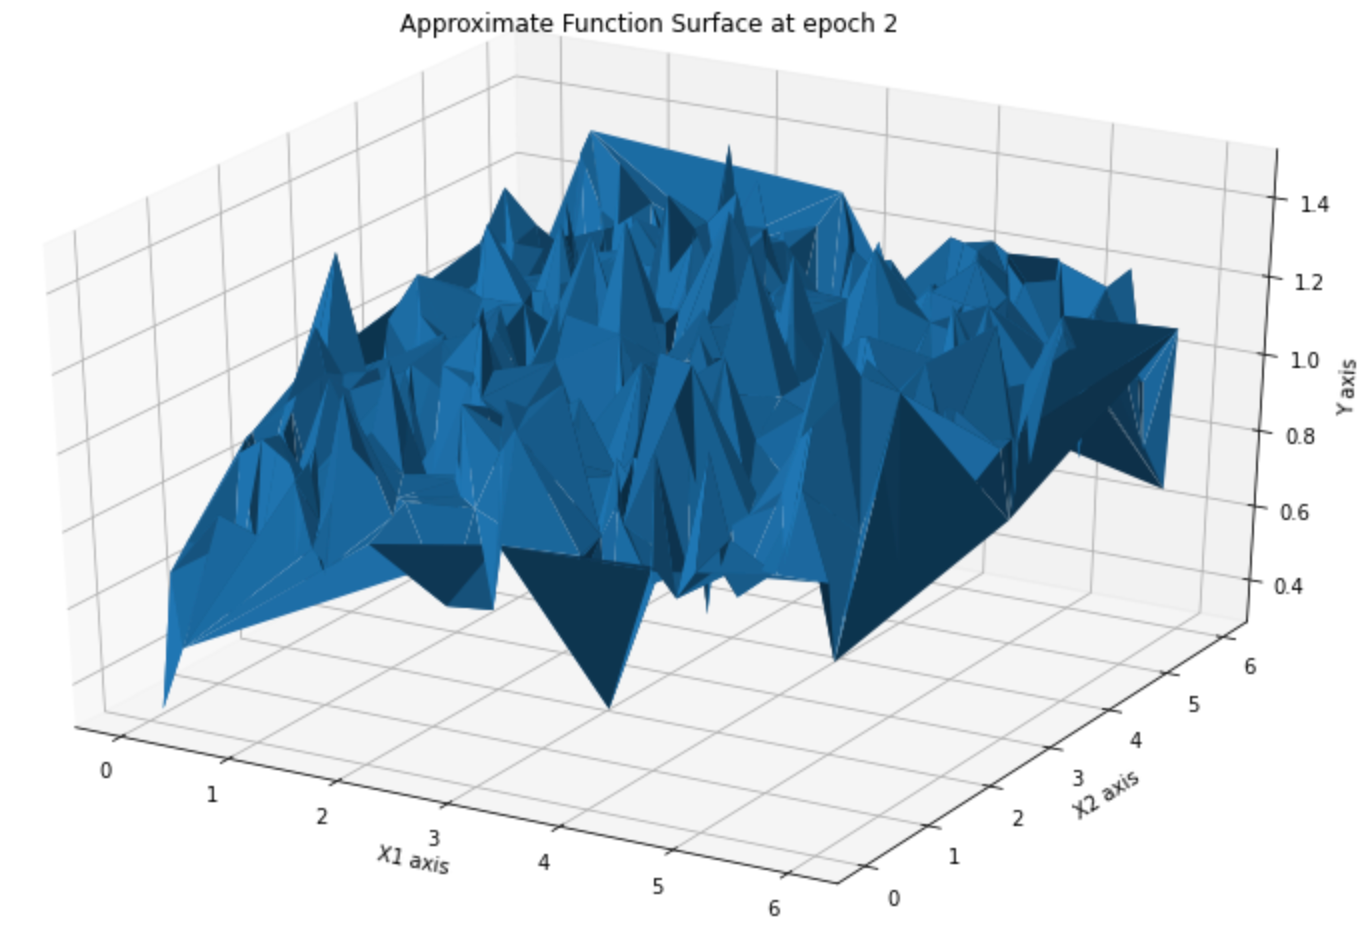
\includegraphics[width=0.8\linewidth]{Ep2.png}
    \captionsetup{justification=centering}
    \caption{Plot of all data applied on the model after 2 epoch}
\end{figure}
\begin{figure}[htbp]
    \centering
    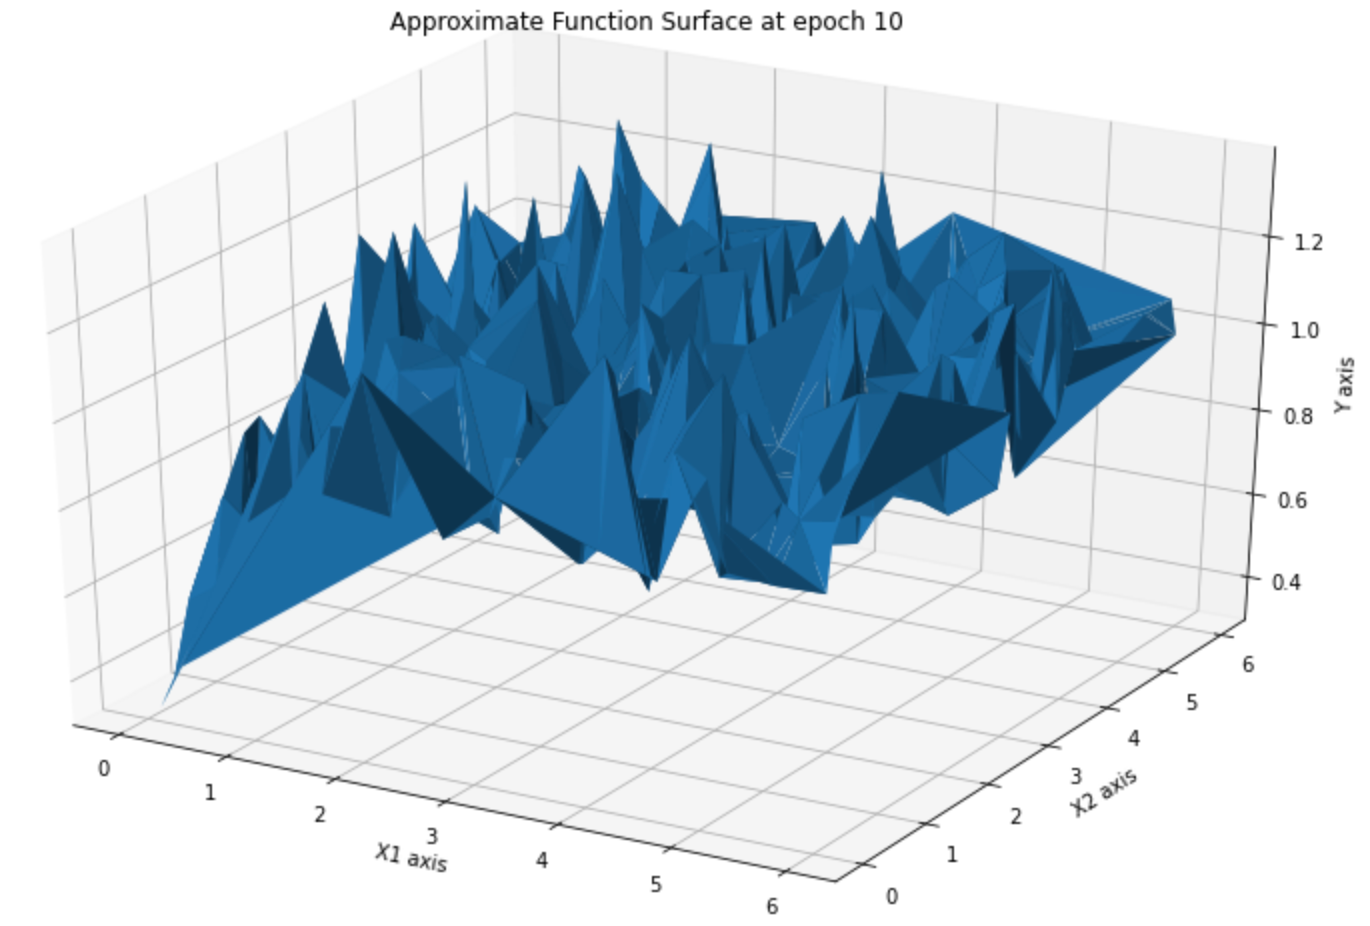
\includegraphics[width=0.8\linewidth]{Ep10.png}
    \captionsetup{justification=centering}
    \caption{Plot of all data applied on the model after 10 epoch}
\end{figure}
\begin{figure}[htbp]
    \centering
    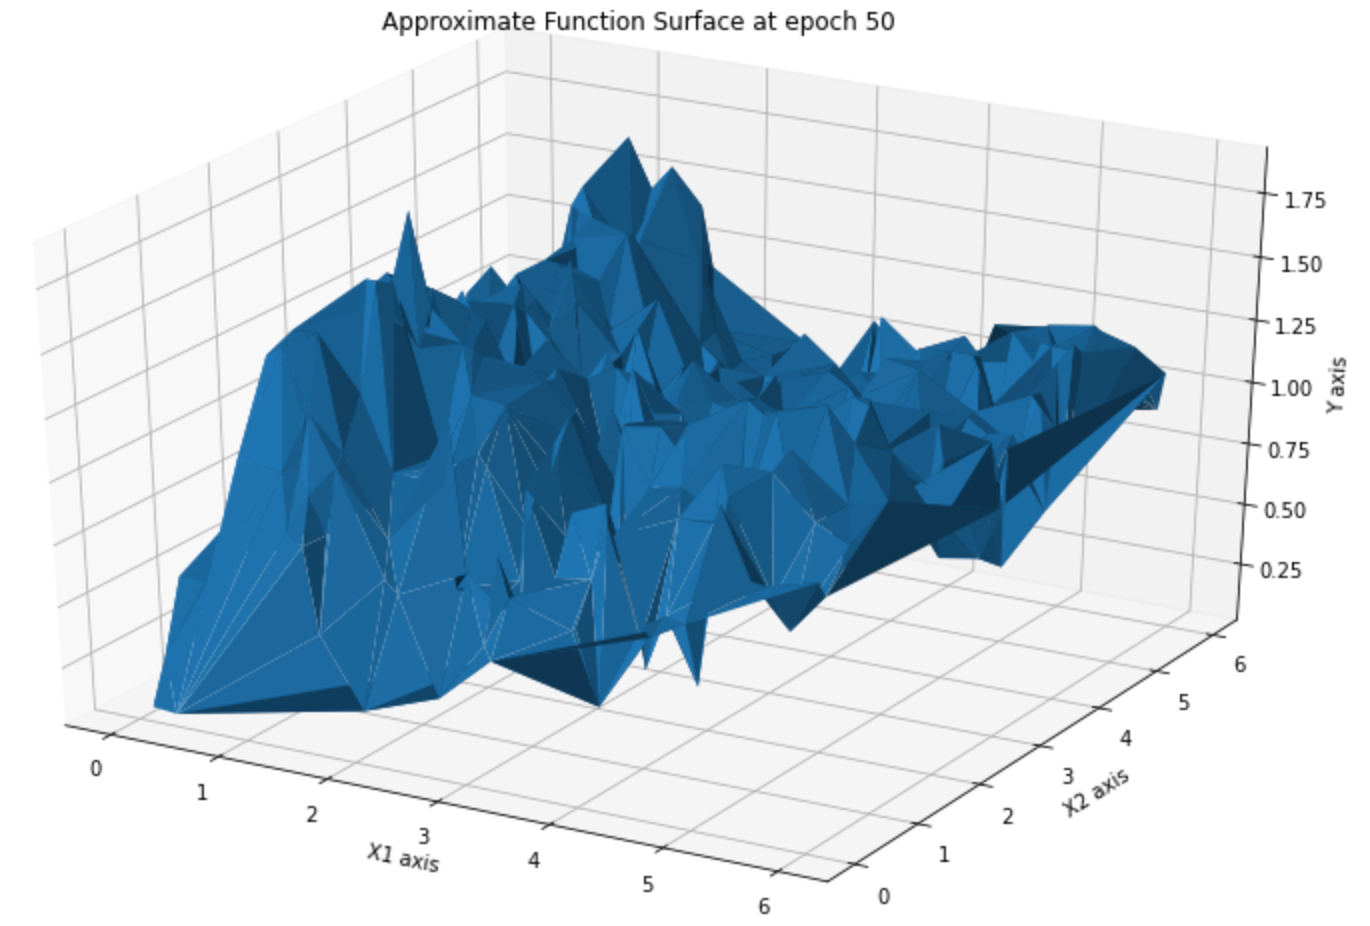
\includegraphics[width=0.8\linewidth]{Ep50.png}
    \captionsetup{justification=centering}
    \caption{Plot of all data applied on the model after 50 epoch}
\end{figure}
\begin{figure}[htbp]
    \centering
    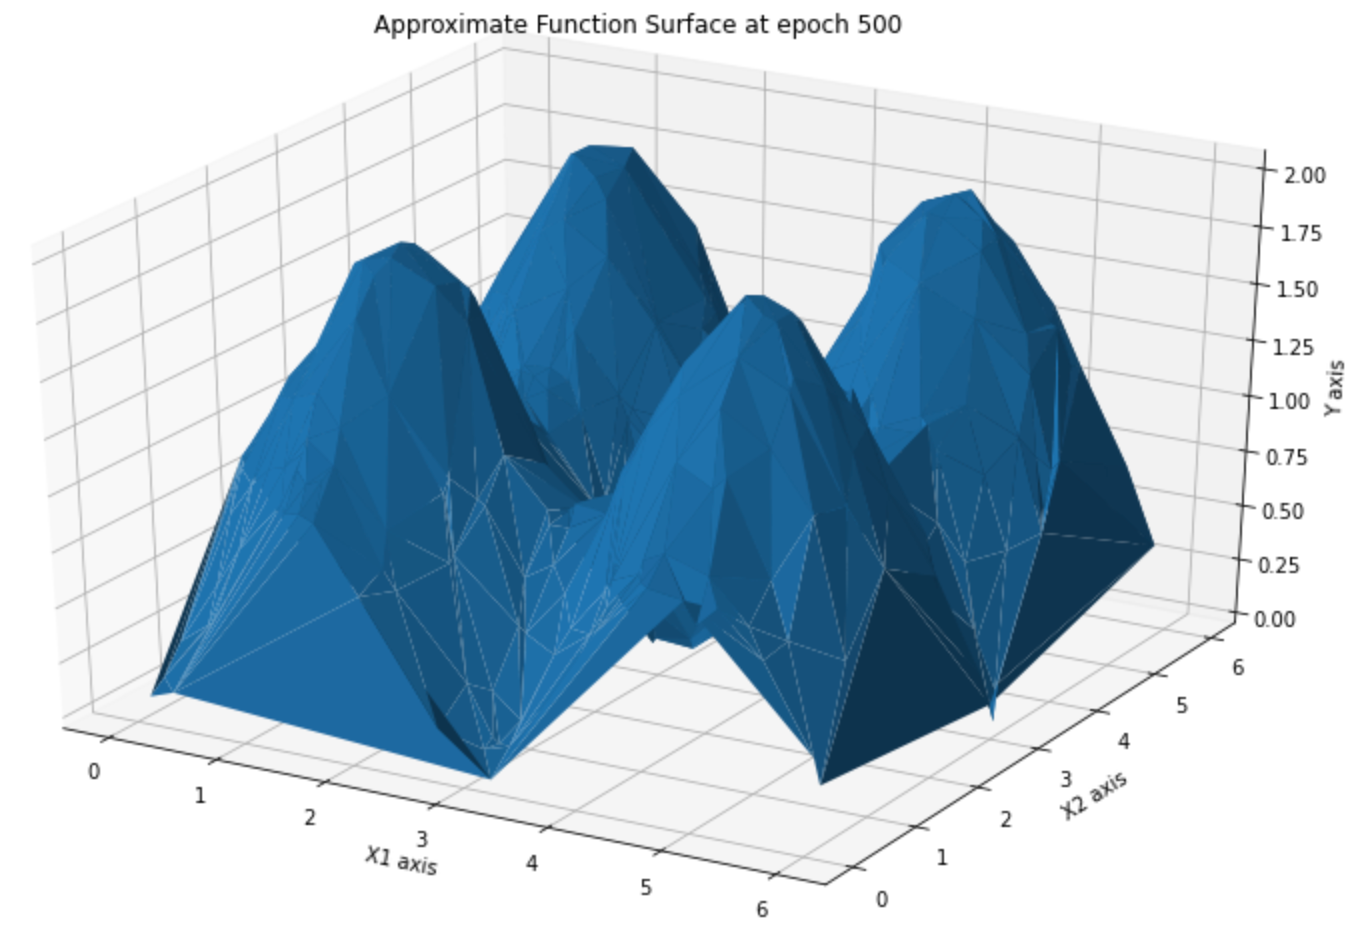
\includegraphics[width=0.8\linewidth]{Ep500.png}
    \captionsetup{justification=centering}
    \caption{Plot of all data applied on the model after 500 epoch}
\end{figure}
\begin{figure}[htbp]
    \centering
    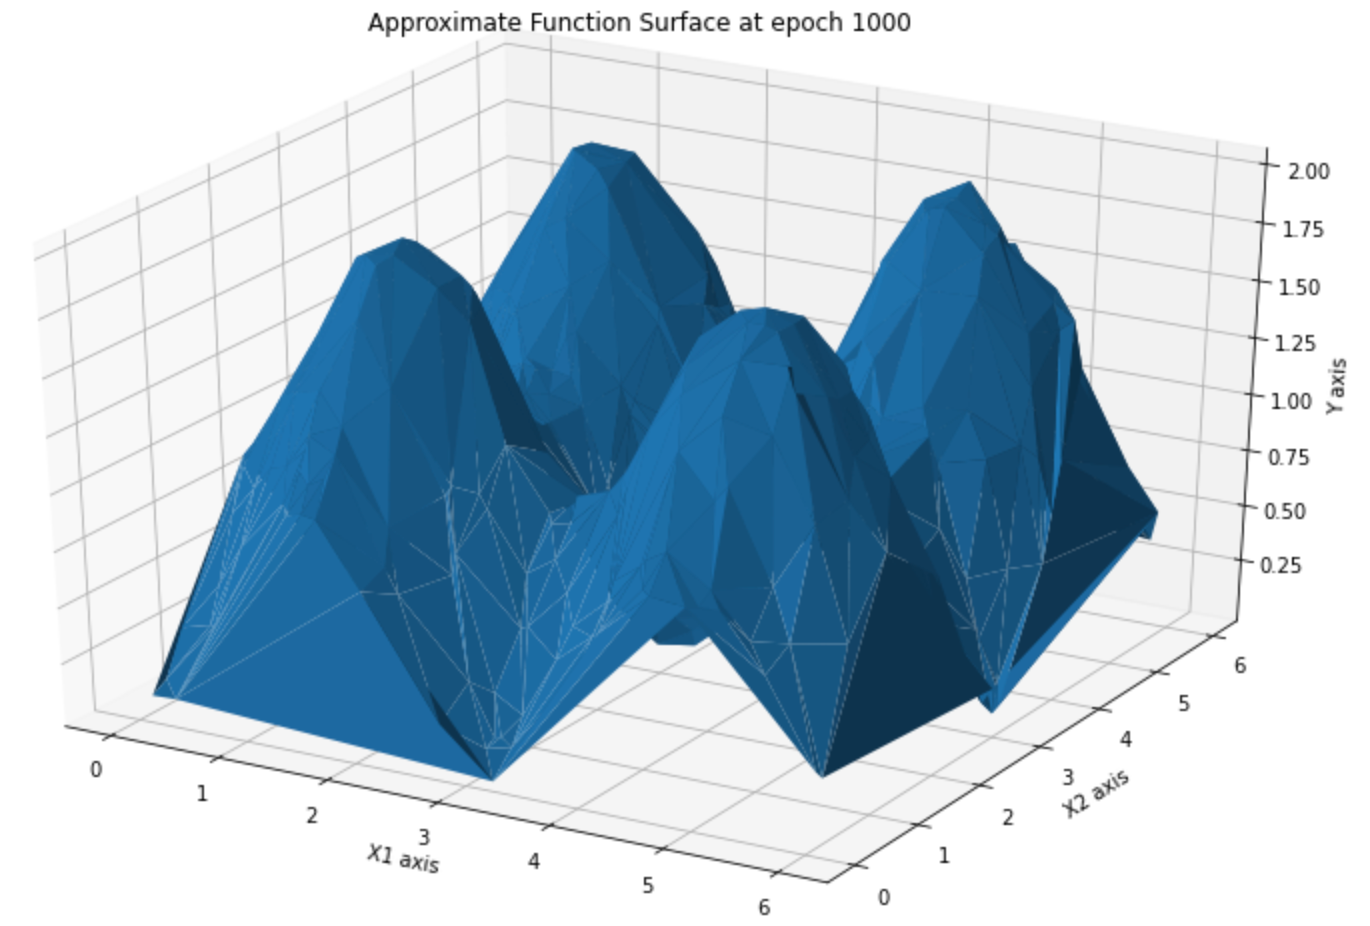
\includegraphics[width=0.8\linewidth]{Ep1000.png}
    \captionsetup{justification=centering}
    \caption{Plot of all data applied on the model after 1000 epoch}
\end{figure}
\begin{figure}[htbp]
    \centering
    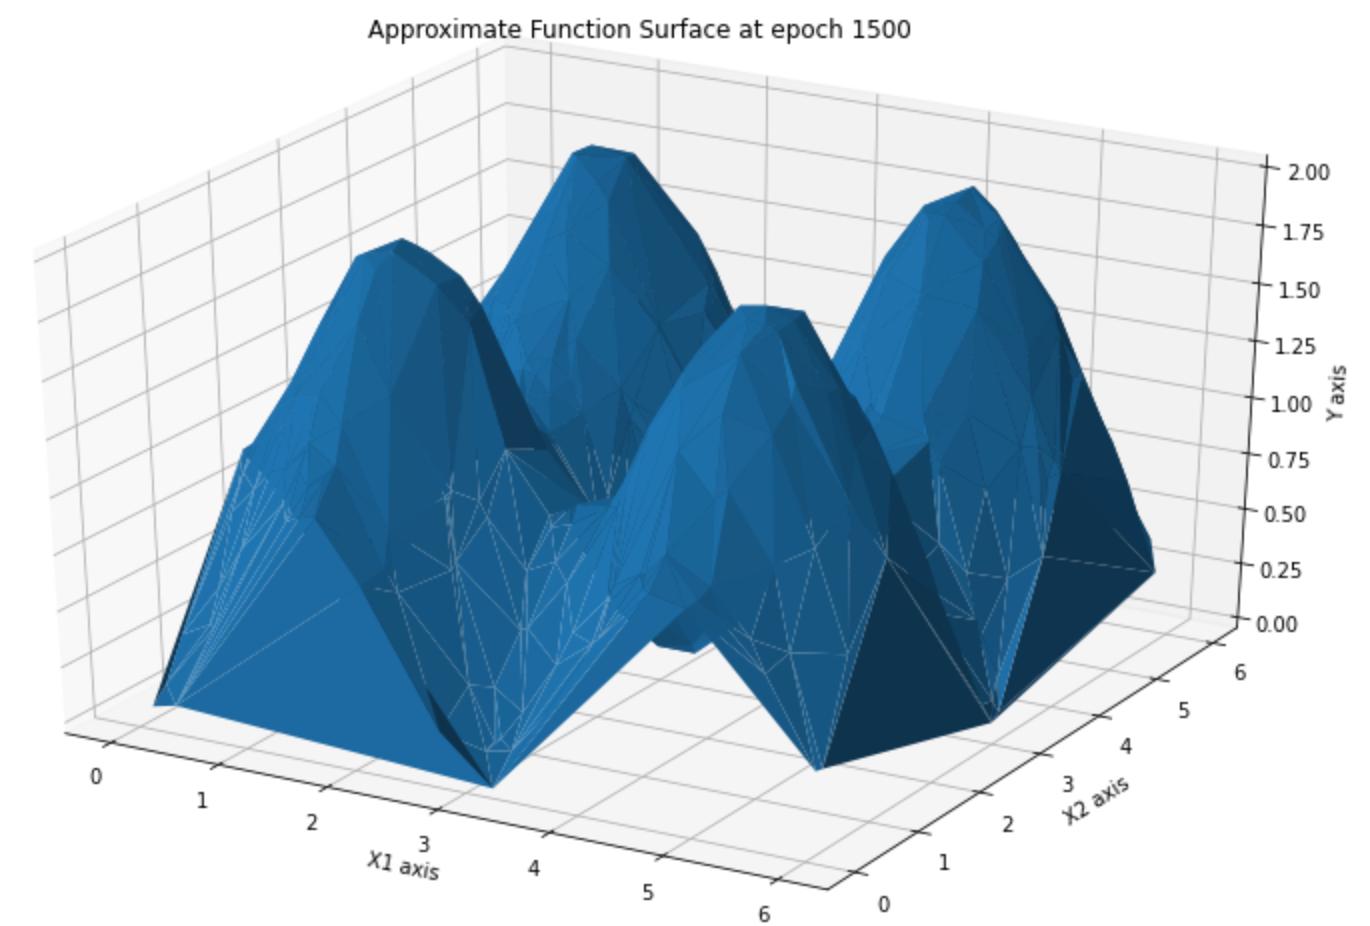
\includegraphics[width=0.8\linewidth]{Ep1500.png}
    \captionsetup{justification=centering}
    \caption{Plot of all data applied on the model after 1500 epoch}
\end{figure}
\begin{figure}[htbp]
    \centering
    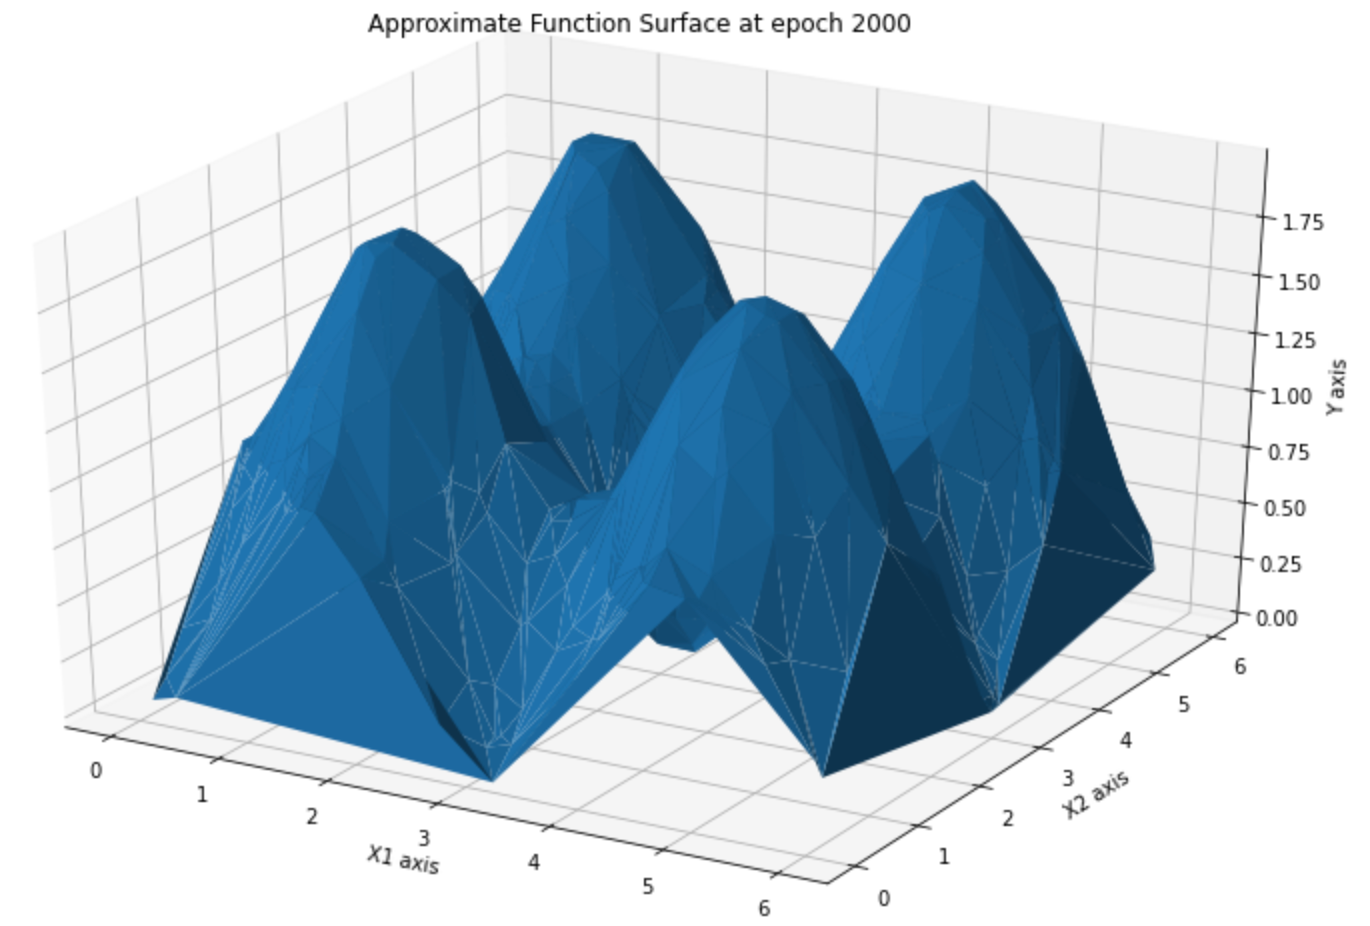
\includegraphics[width=0.8\linewidth]{Ep2000.png}
    \captionsetup{justification=centering}
    \caption{Plot of all data applied on the model after 2000 epoch}
\end{figure}
\newpage
Next I plot the error plot for the t

\subsection{Implementation Details:}

To prevent the model from overfitting (blah blah blah)


raining data, to see how well the training data learns with multiple epochs. We observe that the loss steeply drops within the first few epochs and them asymptotically reaches to a value after which it is not able to learn much, and oscillates around the found local optimum.
\begin{figure}[htbp]
    \centering
    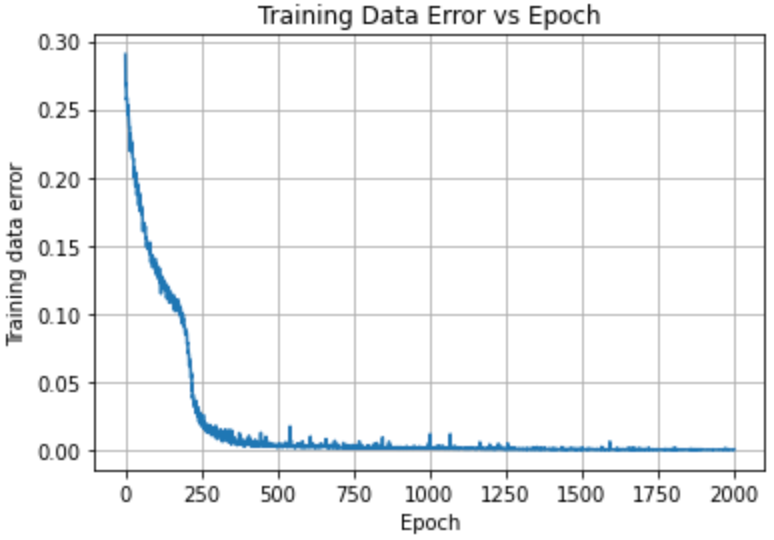
\includegraphics[width=0.8\linewidth]{errvsep.png}
    \captionsetup{justification=centering}
    \caption{Training data error vs Number of epochs}
\end{figure}
\\
The scatter plot after after training the model for 1500 epochs with the above parameters is as follows.\\
\\

\begin{figure}[htbp]
    \centering
    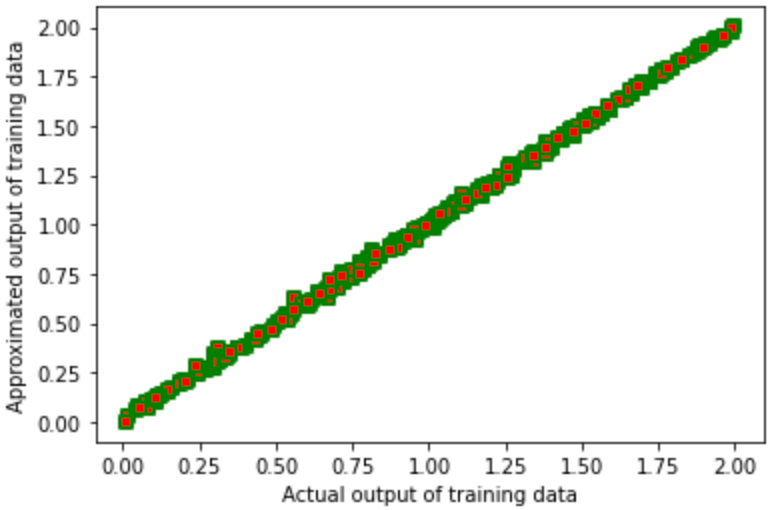
\includegraphics[width=0.8\linewidth]{Scatt.png}
    \captionsetup{justification=centering}
    \caption{Scatter plot of actual output vs model obtained output of training data}
\end{figure}

\subsection{Observations}
\begin{itemize}
    \item As the number of epochs increases, the average error decreases. After a point, the output just oscillates around the local optimum.
    \item Train average loss: 0.00167
    \item Test average loss: 0.00114
    \item The scatter plot showa that the data points almost lie along the $x=y$ line, showing the model has learnt well.
    \item The final plot obtained at 2000 epochs almost resembles the actual function plot, except it is more sharper at the edges.
    \item The validation loss varies with the epochs as follows:
    \subitem Validation average loss at epoch 0000: 0.217057
    \subitem Validation average loss at epoch 0100: 0.106351
	\subitem Validation average loss at epoch 0200: 0.050664
	\subitem Validation average loss at epoch 0300: 0.005119
	\subitem Validation average loss at epoch 0400: 0.006670
	\subitem Validation average loss at epoch 0500: 0.002086
	\subitem Validation average loss at epoch 0600: 0.001214
	\subitem Validation average loss at epoch 0700: 0.001714
	\subitem Validation average loss at epoch 0800: 0.001274
	\subitem Validation average loss at epoch 0900: 0.001025
	\subitem Validation average loss at epoch 1000: 0.000955
	\subitem Validation average loss at epoch 1100: 0.000678
	\subitem Validation average loss at epoch 1200: 0.000656
	\subitem Validation average loss at epoch 1300: 0.000648
	\subitem Validation average loss at epoch 1400: 0.000698
	\subitem Validation average loss at epoch 1500: 0.000476
	\subitem Validation average loss at epoch 1600: 0.003656
	\subitem Validation average loss at epoch 1700: 0.000401
	\subitem Validation average loss at epoch 1800: 0.000398
	\subitem Validation average loss at epoch 1900: 0.000314
	\item Final Train average loss: 0.00041
	\item Final Test average loss: 0.00031
\end{itemize}


\section{Classifying Image Data}

The images in the dataset given to us have been mapped to features of dimension 60. 
The features are then fed into our Multi Layer Feed Forward Neural Network model to classify the images into five 
distinct classes. The architecture of our model is given in Section 1. We replace the last layer of the model with a 
linear layer containing five output nodes. The output nodes are the logits of the image belonging to each of the
distinct classes. 

We have to compare the performance and the number of epochs taken for convergence for different weight update algorithms such
as delta, generalized delta and Adam. Delta rule is simple stochastic gradient descent with momentum of 0. Generalised delta contains non zero momentum value
Adam algorithm calculates an exponential moving average of the gradient and the squared gradient, and the parameters beta1 and beta2 control the decay rates of these moving averages.

\subsection{Hyper Parameter Optimization}

We tune the hyperparameters such as learning rate, number of neurons in hidden layer 1, number of neurons in hidden layer 2 in our experiments.
We use the validation data to tune the hyperparameters. We use grid search method to tune our hyperparameters.

\subsection{Results}

\subsubsection{Comparison of weight update rules using same hyperparameters}

We choose a fixed set of hyperparameters for our model. We use the same weight initialisation 
while comparing the different weight update rule. We plot the training loss, validation loss, training accuracy and validation accuracy with respect to epochs.
The hyperparameters that we choose for the model is 64 as the number of neurons in hidden layer 1, 64 as the number of neurons in hidden layer 2, 1e-4 as the learning rate
and 0.8 as the momentum.

\begin{figure}%
    \centering
    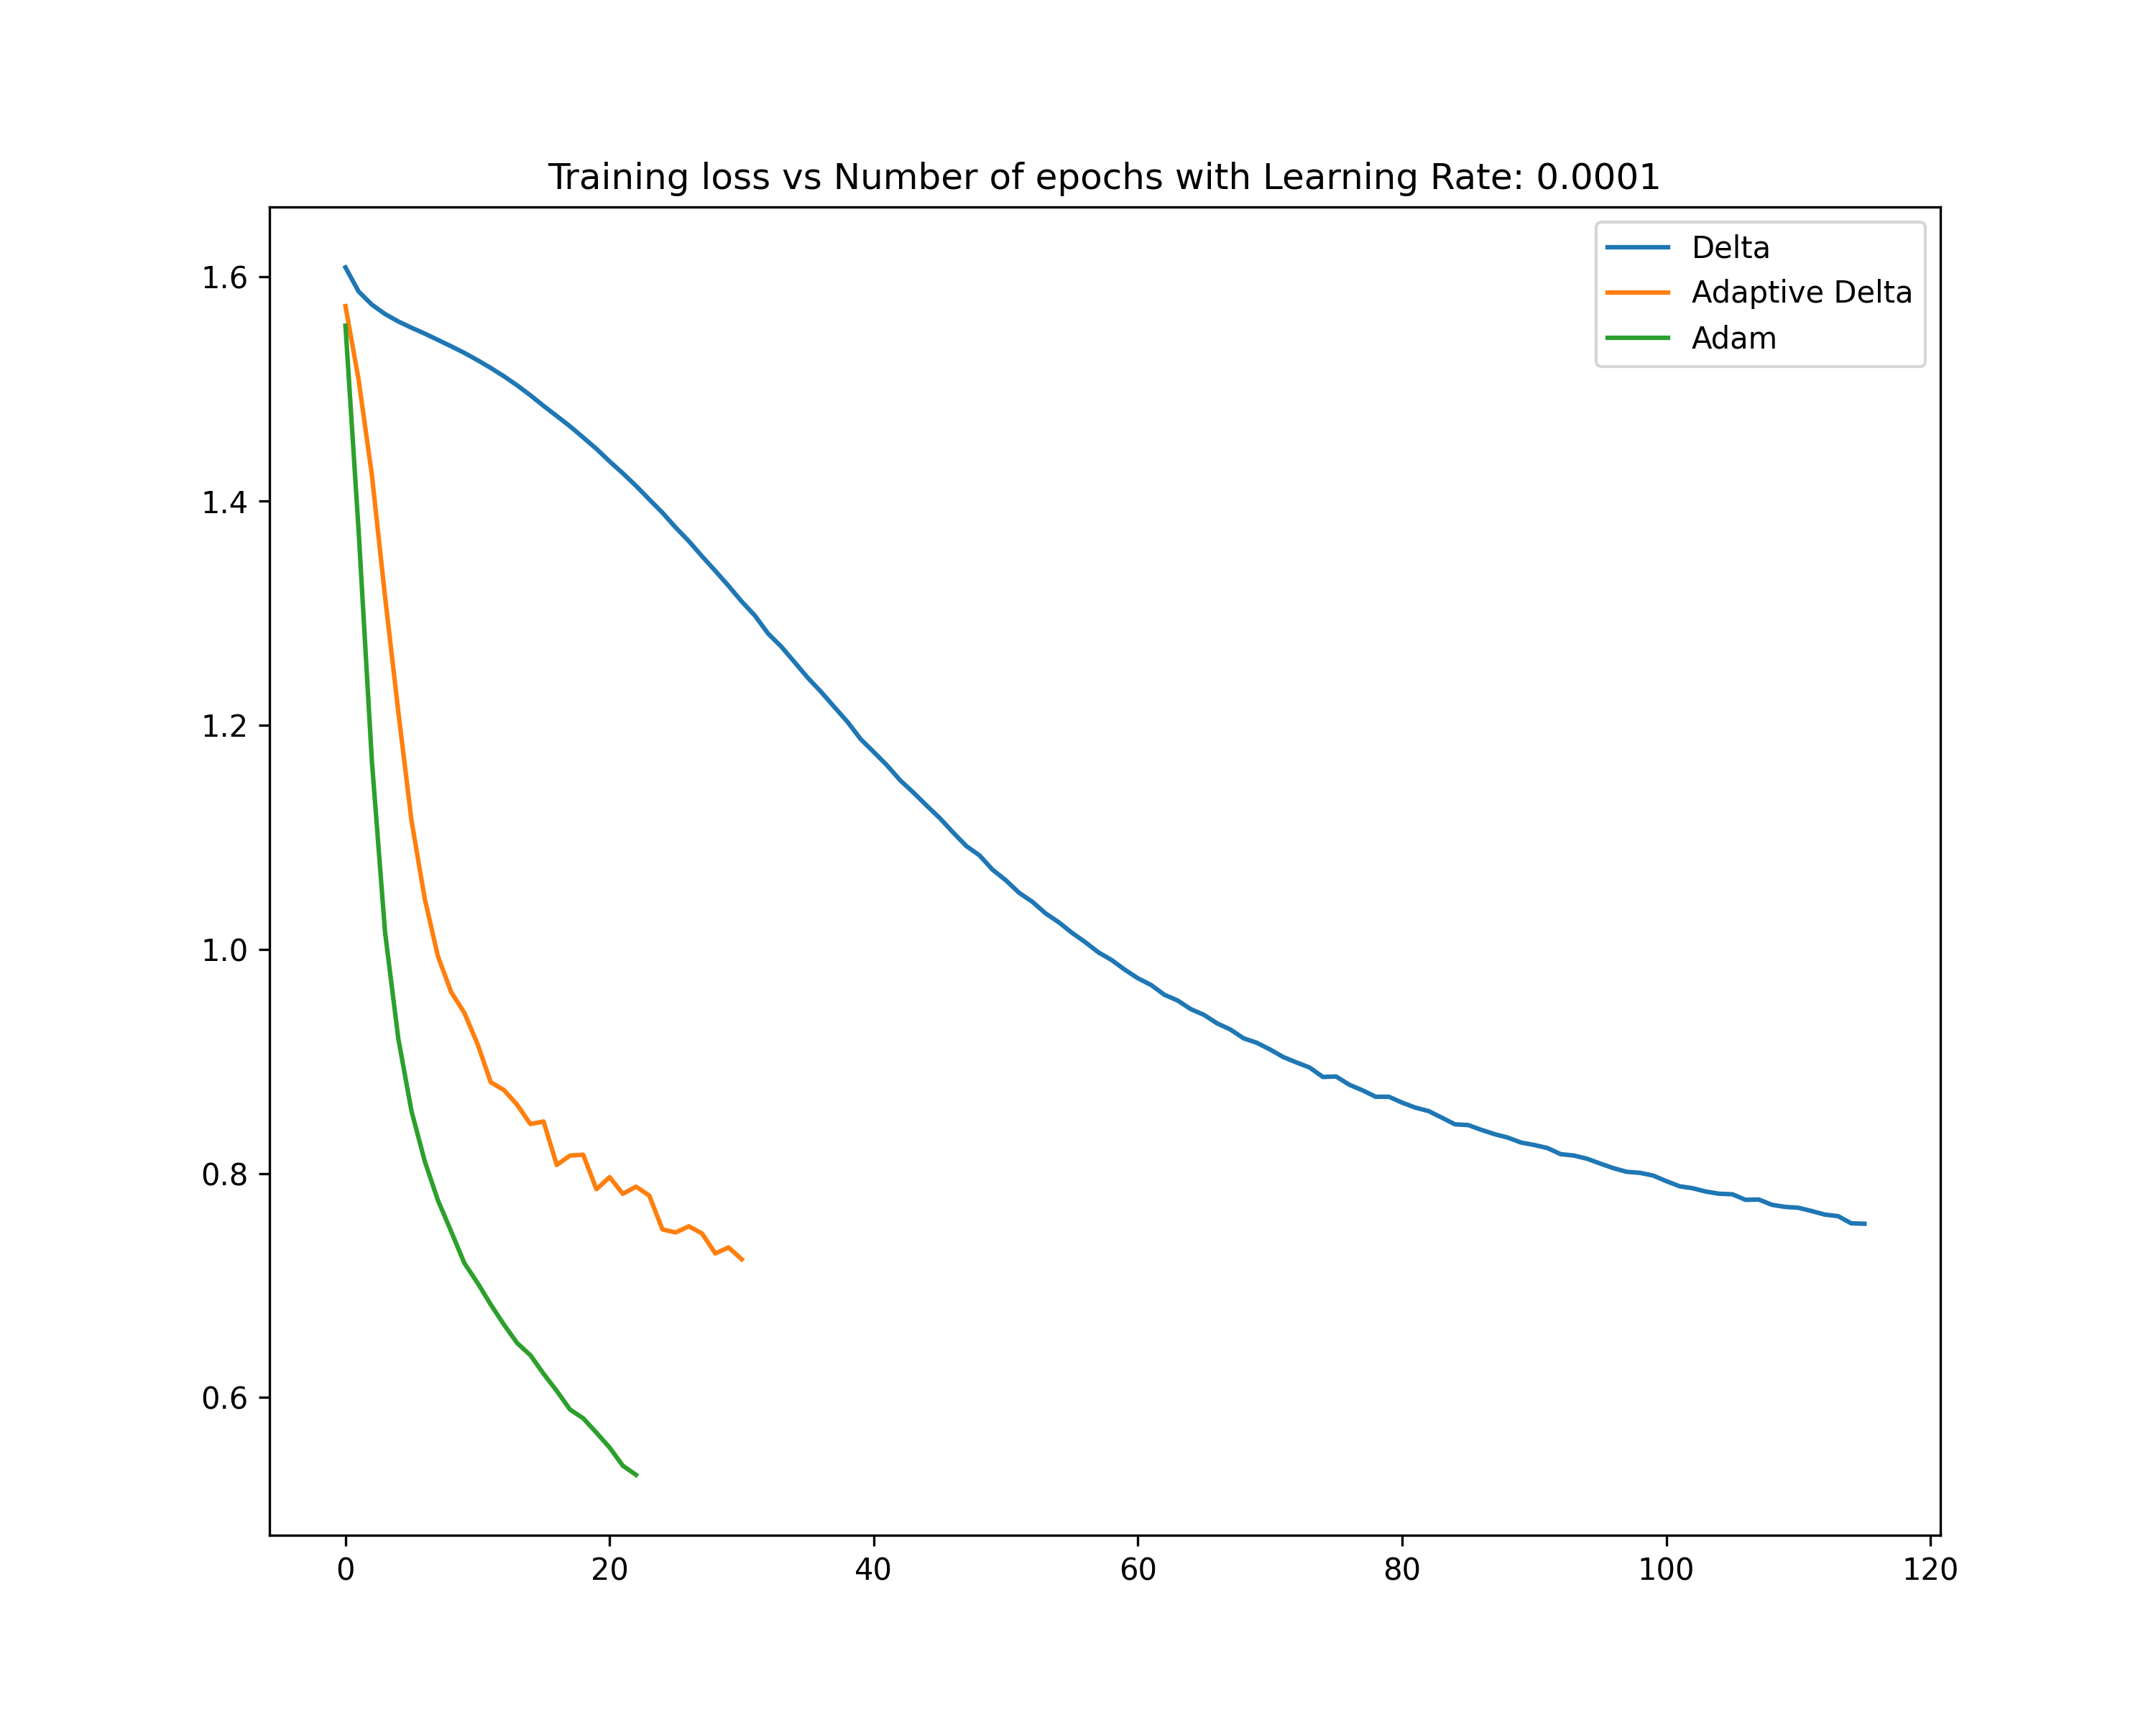
\includegraphics[scale=0.6]{training_loss_0.0001.png}%
    \caption{Comparing the training loss vs number of epochs for different weight update rules utilising same hyperparameters}%
    \label{fig:8}%
\end{figure}

\begin{figure}%
    \centering
    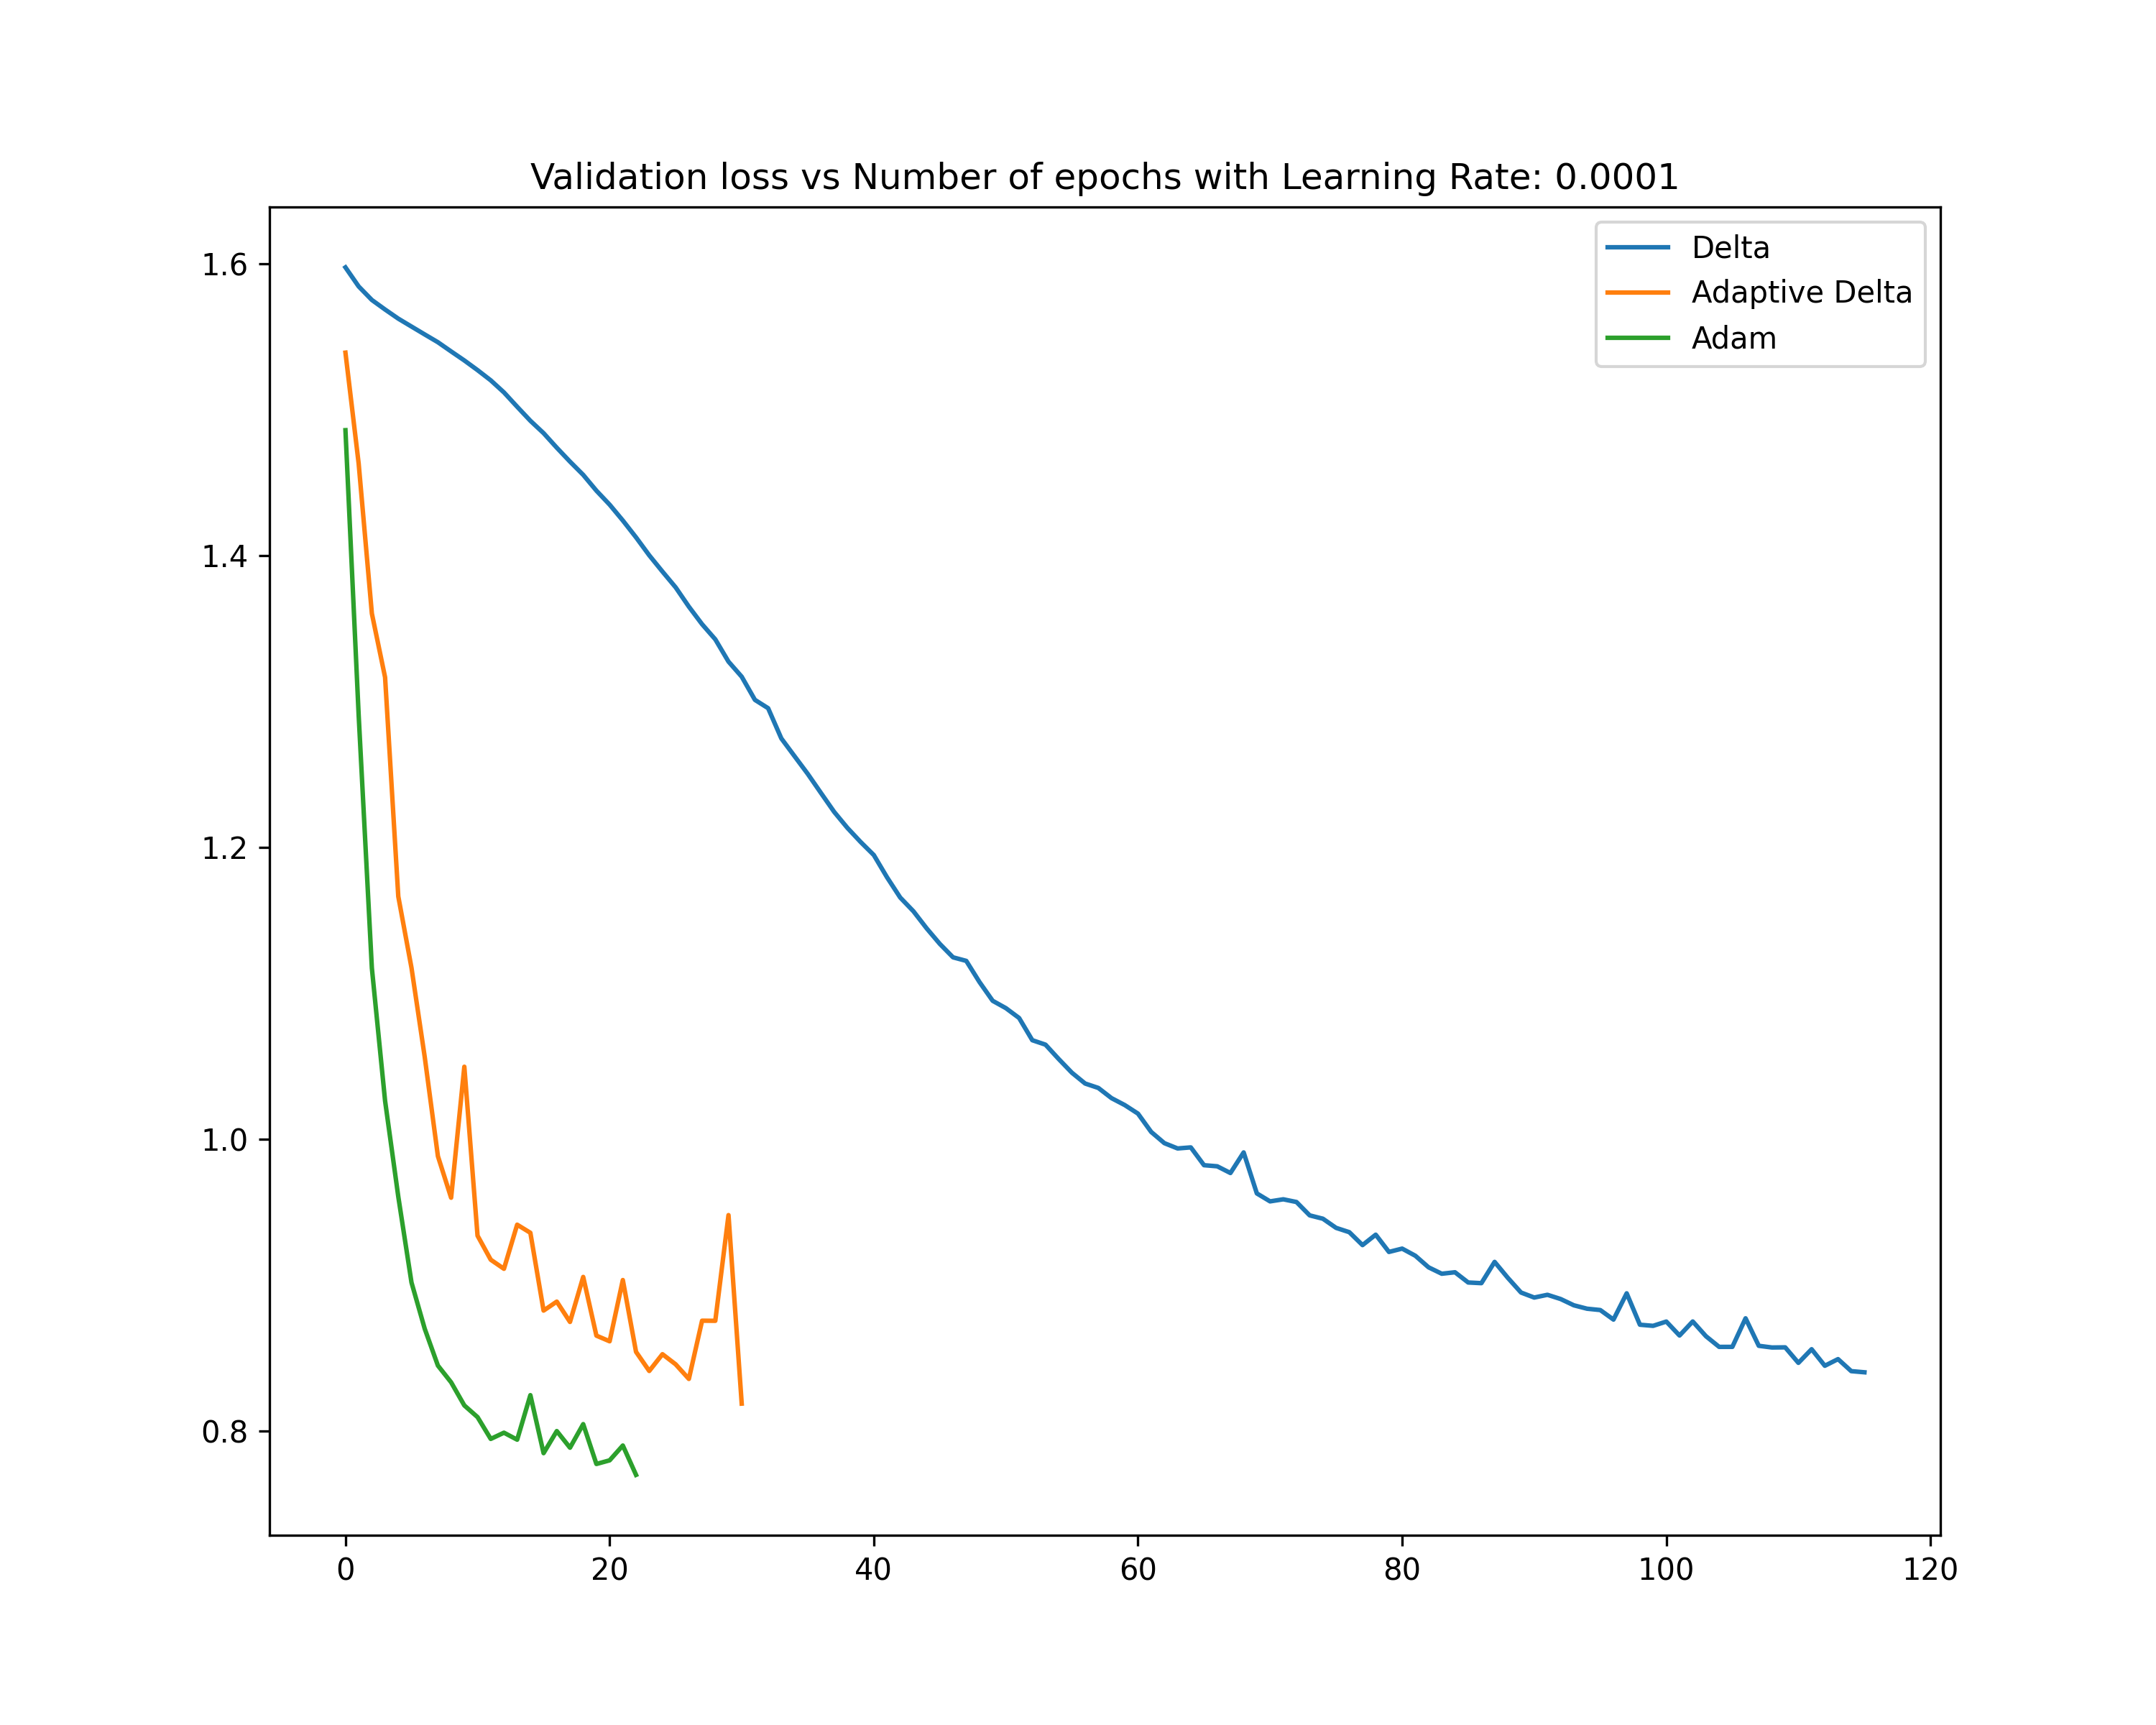
\includegraphics[scale=0.6]{validation_loss_0.0001.png}%
    \caption{Comparing the validation loss vs number of epochs for different weight update rules but utilising the same hyperparameters}%
    \label{fig:9}%
\end{figure}

\begin{figure}%
    \centering
    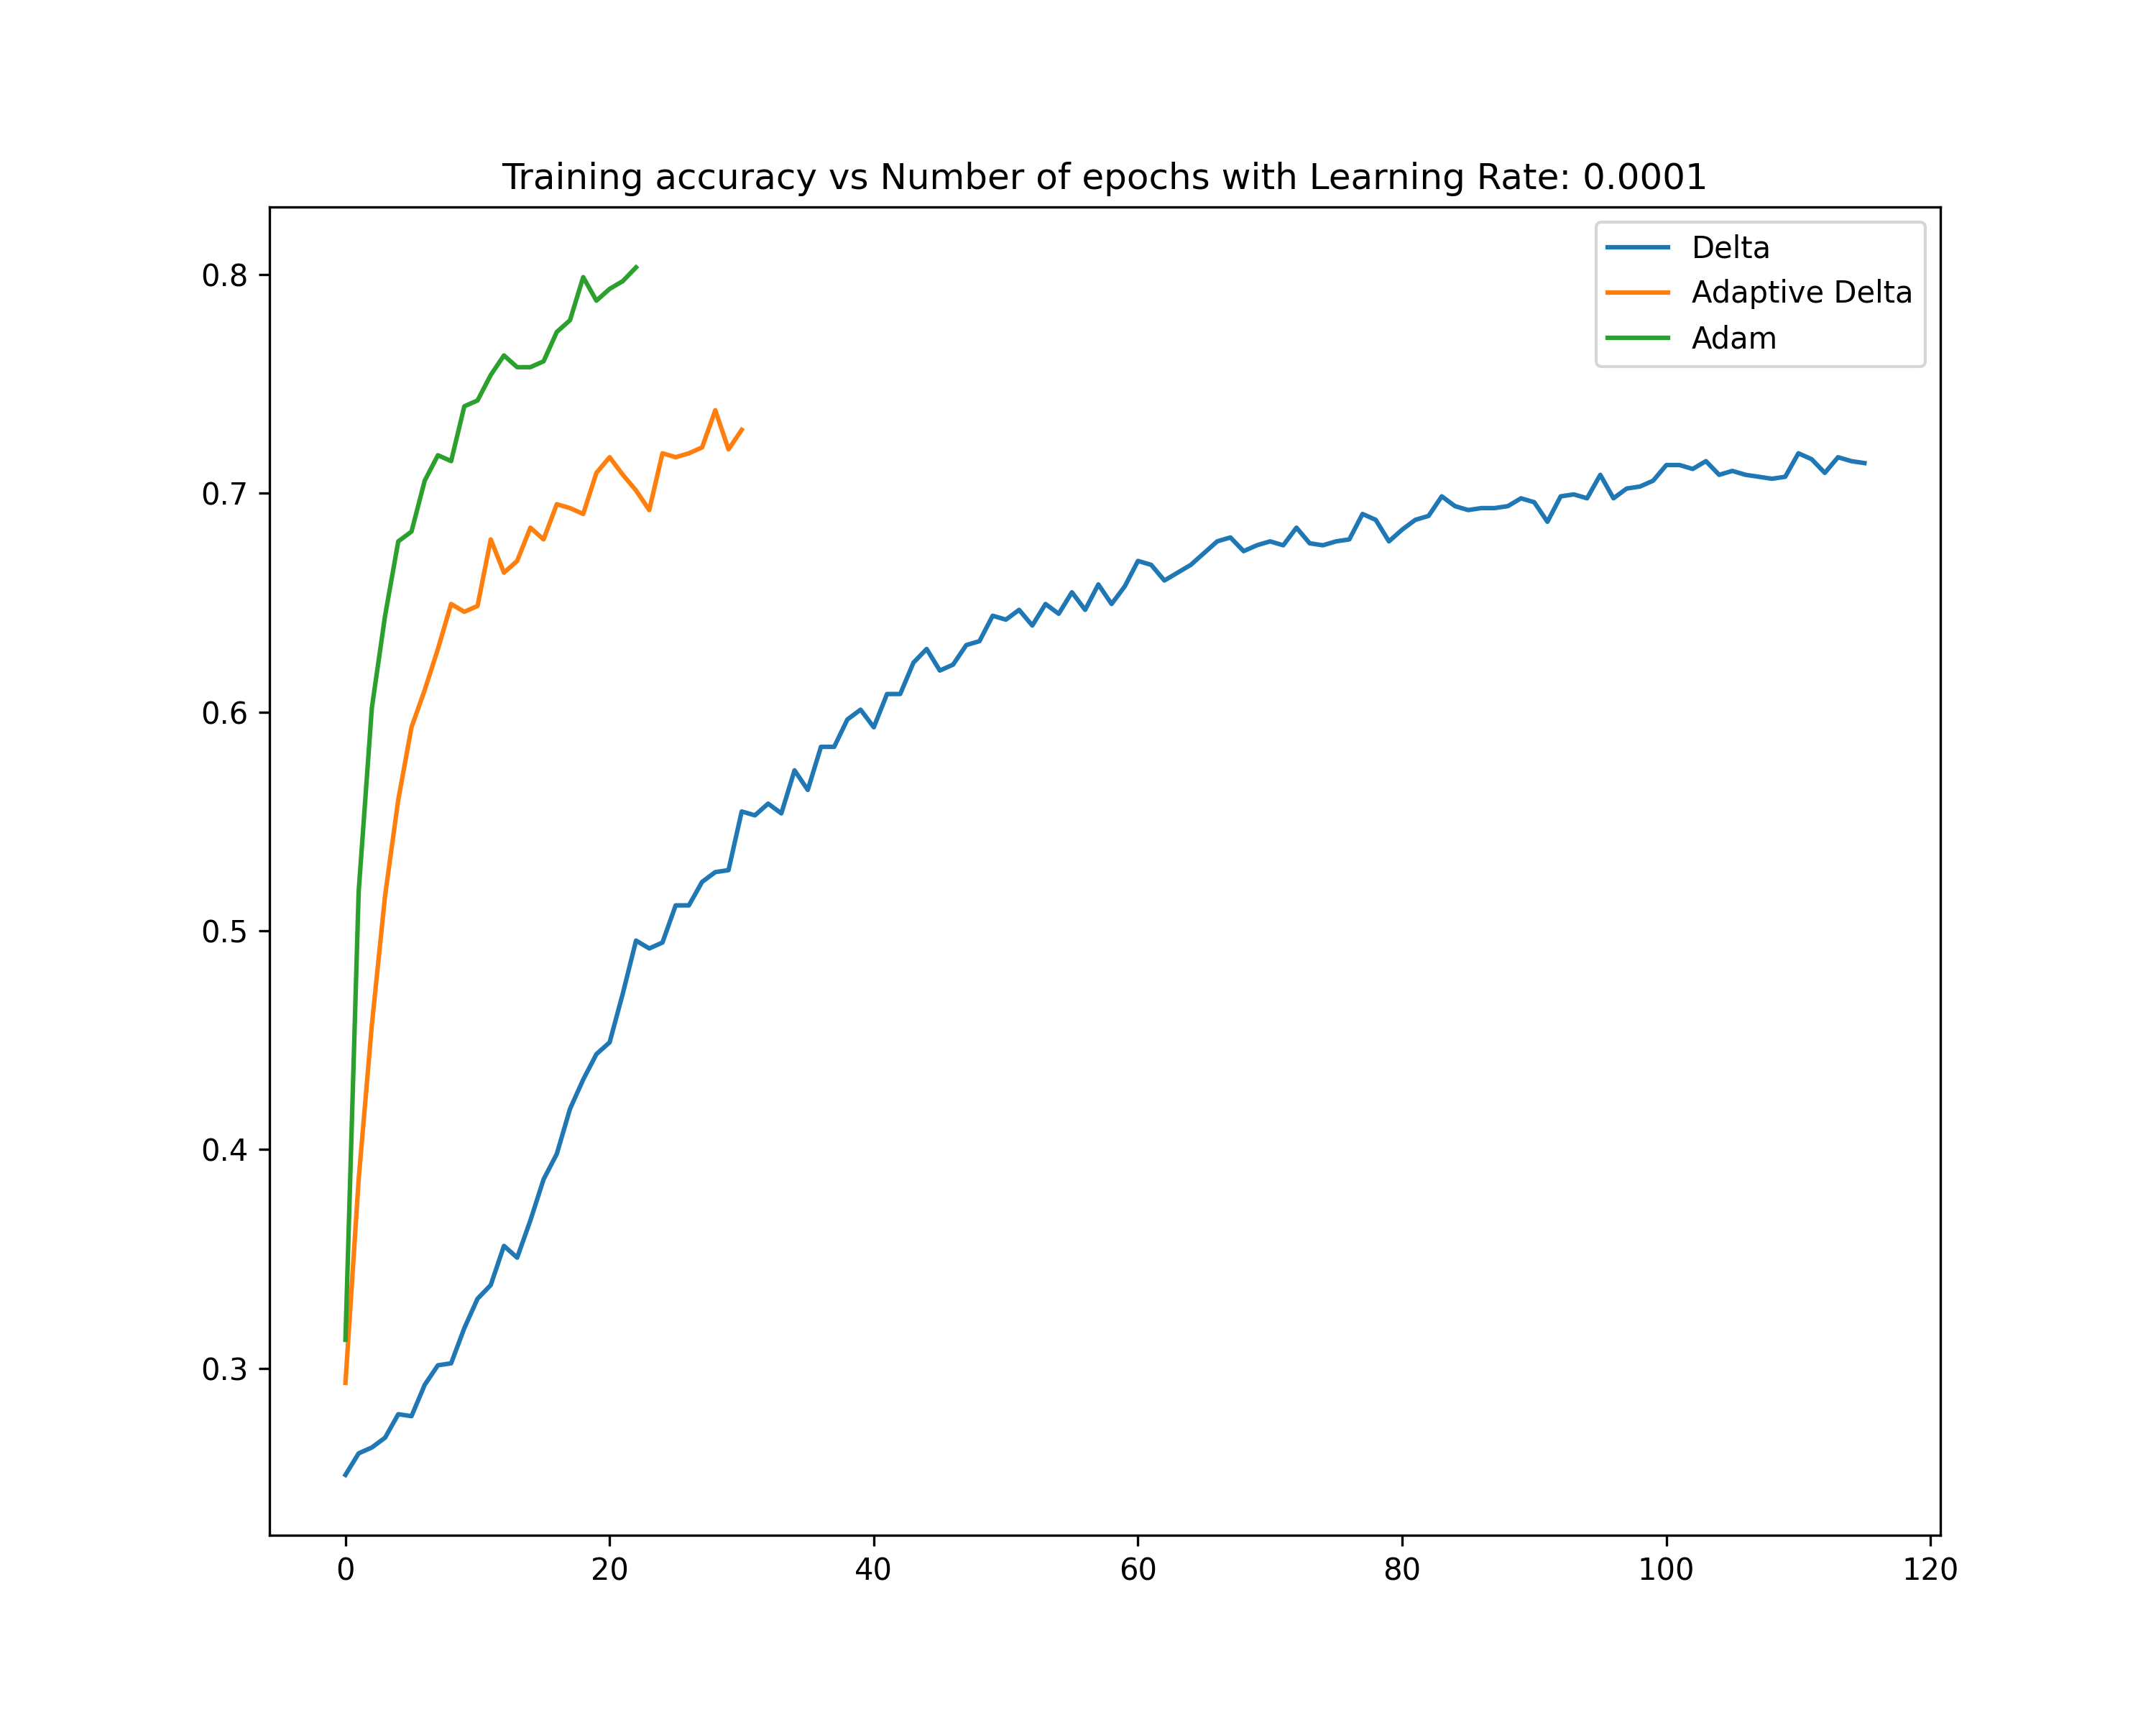
\includegraphics[scale=0.6]{training_accuracy_0.0001.png}%
    \caption{Comparing the training accuracy vs number of epochs for different weight update rules but utilising the same hyperparameters}%
    \label{fig:10}%
\end{figure}

\begin{figure}%
    \centering
    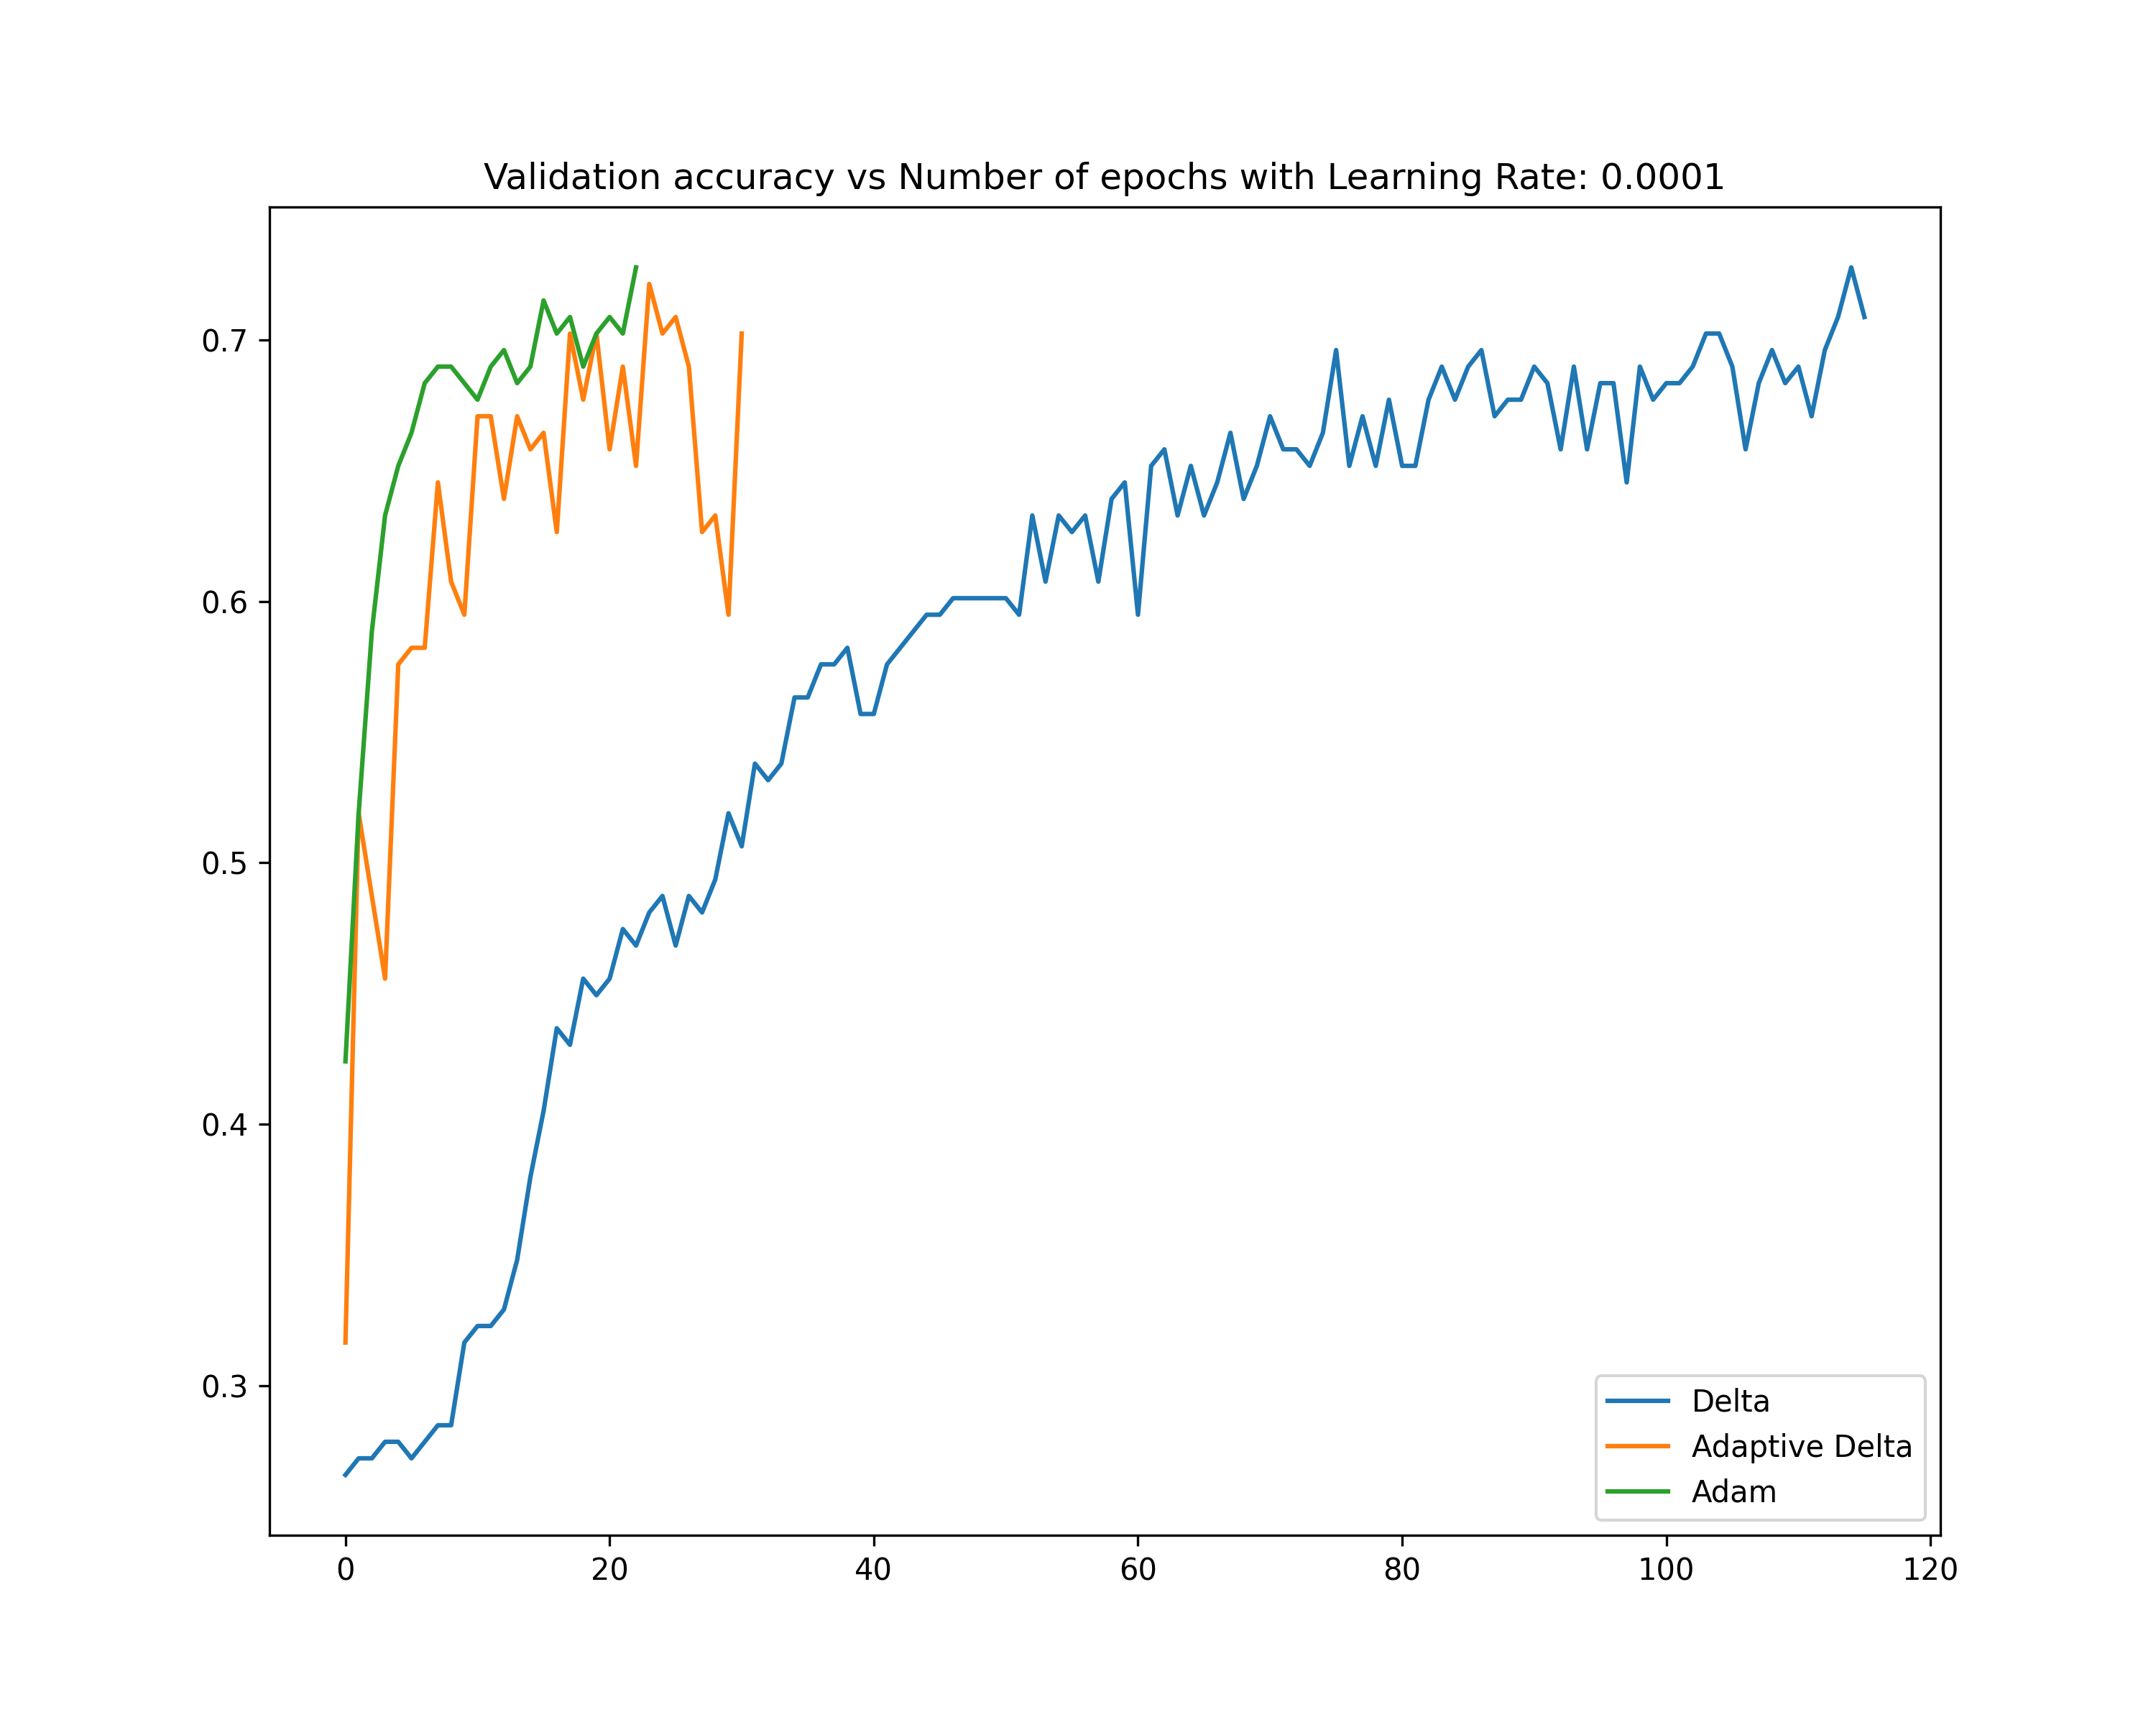
\includegraphics[scale=0.6]{validation_accuracy_0.0001.png}%
    \caption{Comparing the validation accuracy for different weight update rules but utilising the same hyperparameters}%
    \label{fig:11}%
\end{figure}


\subsubsection{Confusion Matrix and Training Loss for optimum hyperparameters}

We optimise the hyperparameters using the validation data. 
Using these optimum hyperparameters, we plot the confusion matrix and the training loss variation for different weight update rules. 

\begin{figure}[H]
    \centering
    \subfloat[\centering Training Data]{{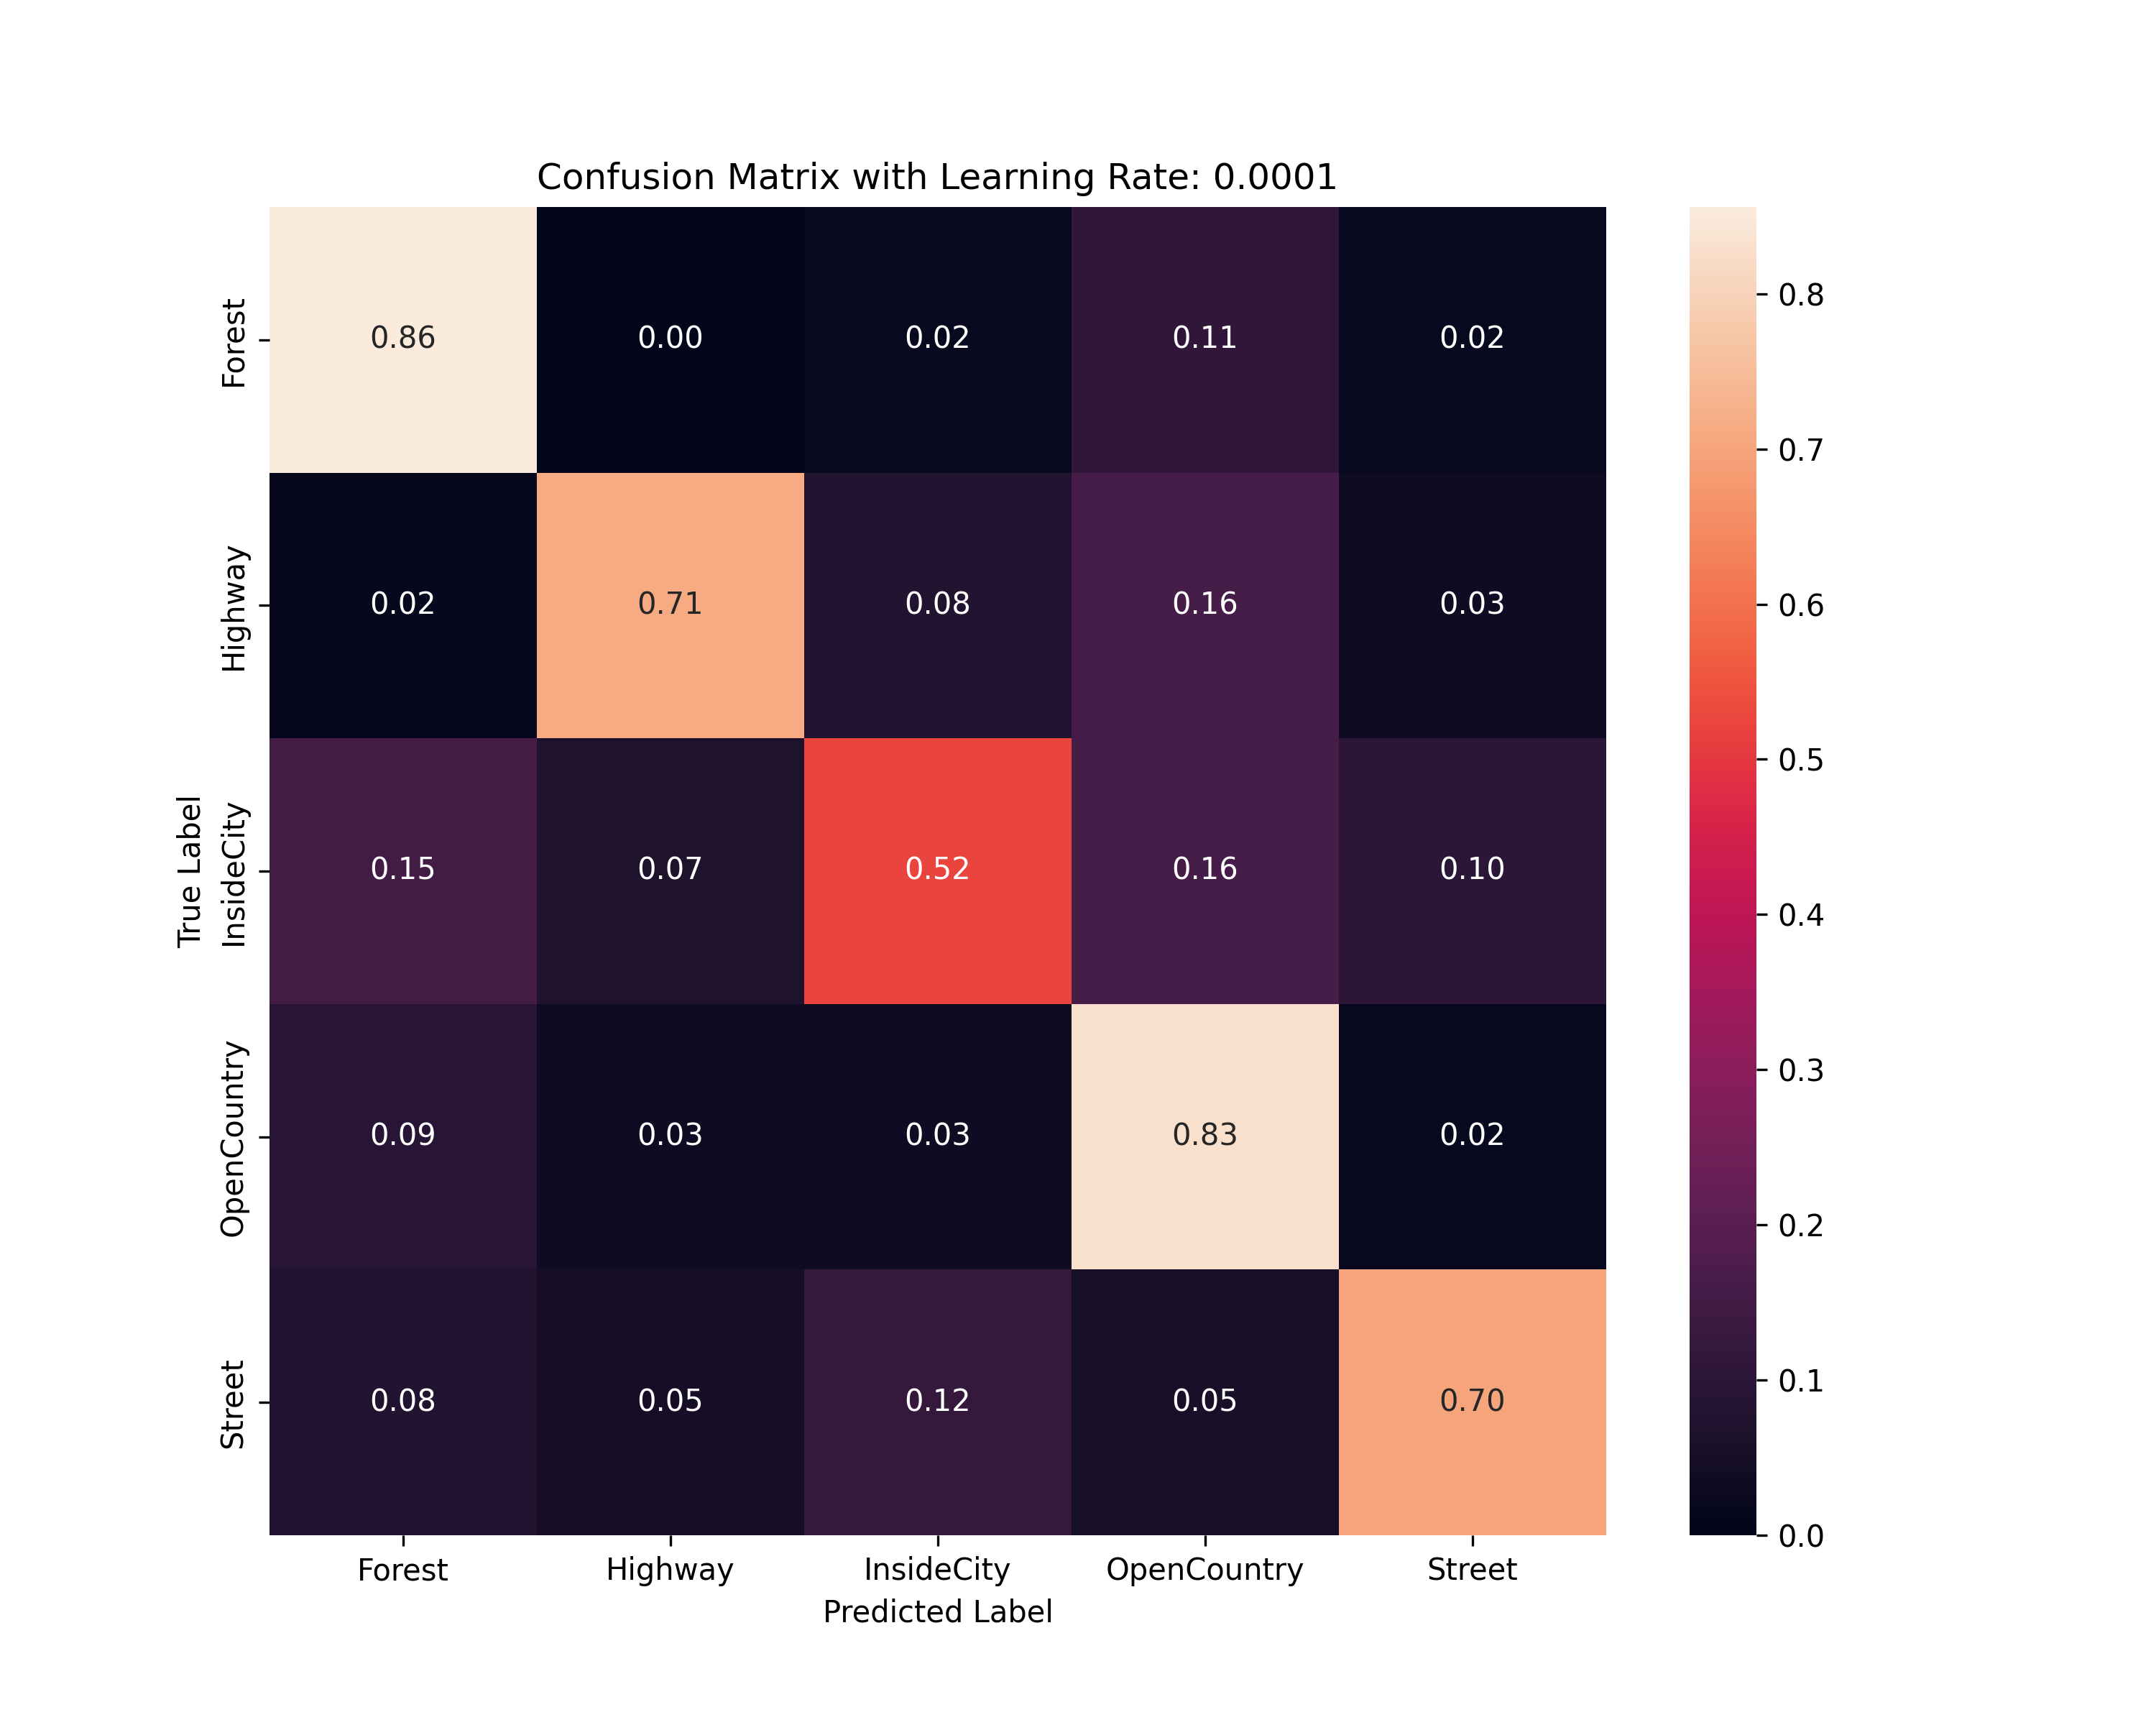
\includegraphics[width=6.5cm]{confusion_matrix_model_delta_train_0.0001.png} }}%
    \qquad
    \subfloat[\centering Test Data]{{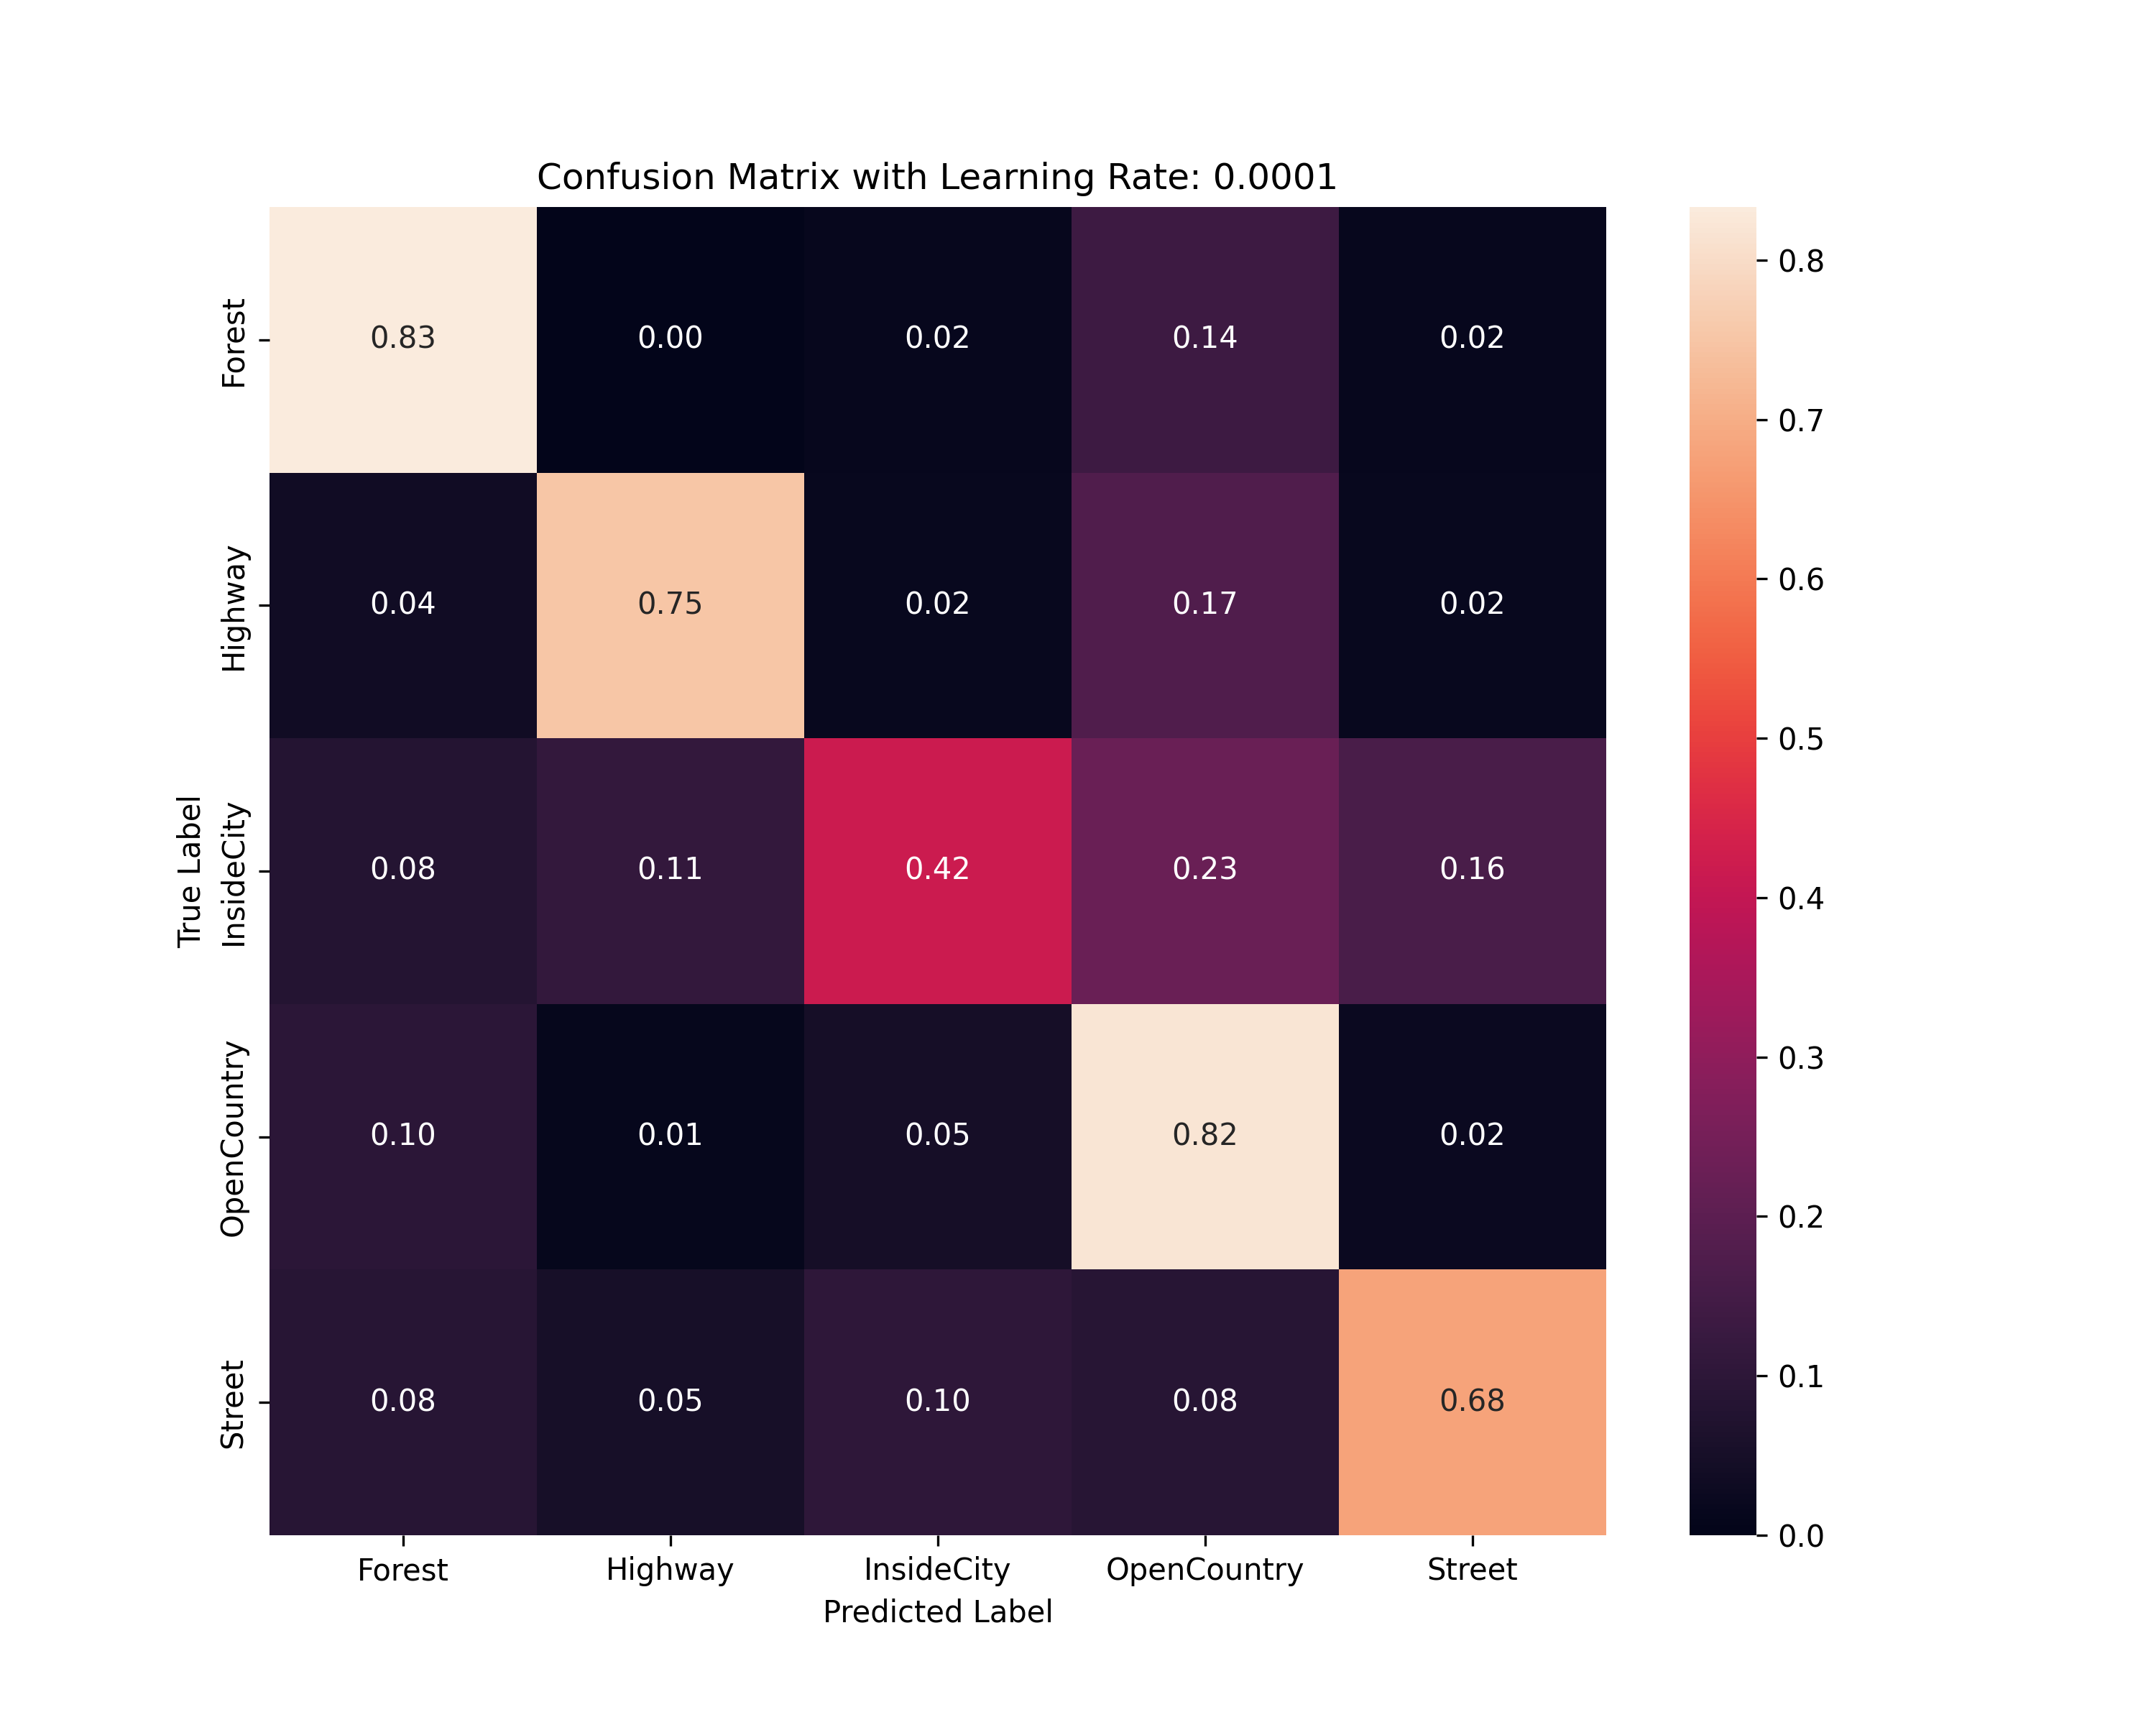
\includegraphics[width=6.5cm]{confusion_matrix_model_delta_test_0.0001.png} }}%
    \caption{Confusion Matrix for Delta Rule on training and test dataset}%
    \label{fig:1}
\end{figure}

\begin{figure}[H]
    \centering
    \subfloat[\centering Training Data]{{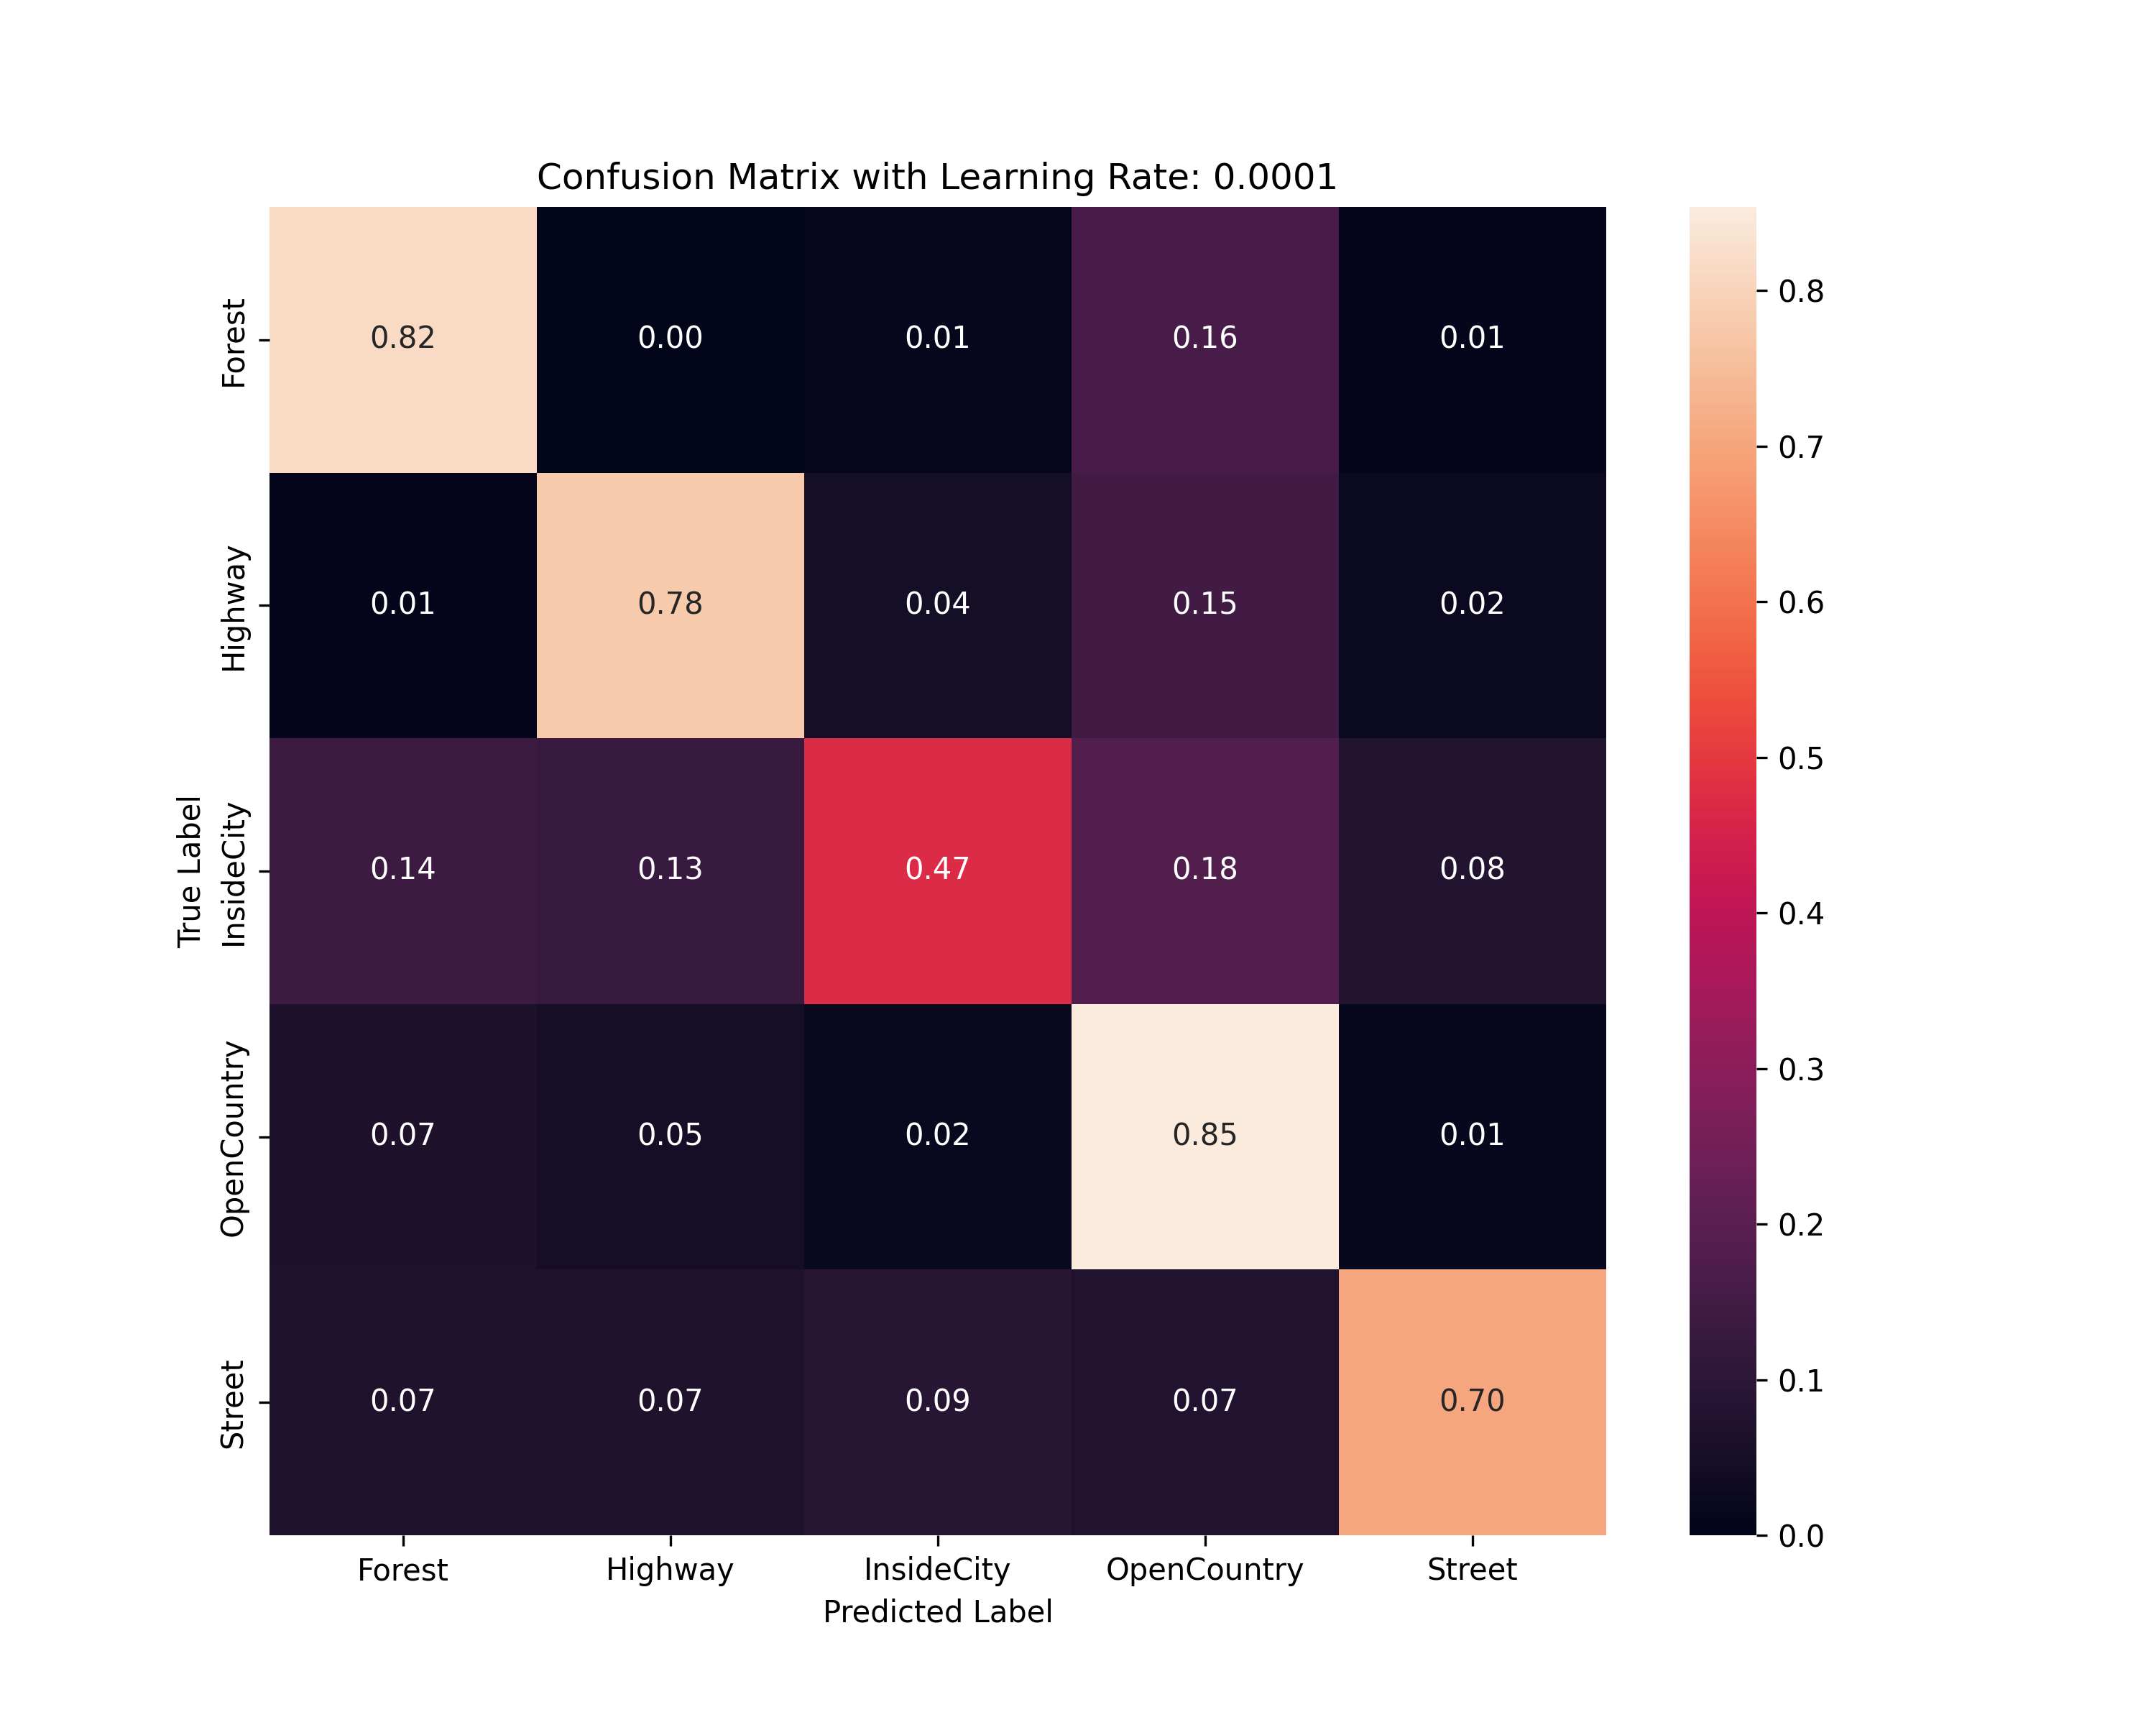
\includegraphics[width=6cm]{confusion_matrix_model_ada_delta_train_0.0001.png} }}%
    \qquad
    \subfloat[\centering Test Data]{{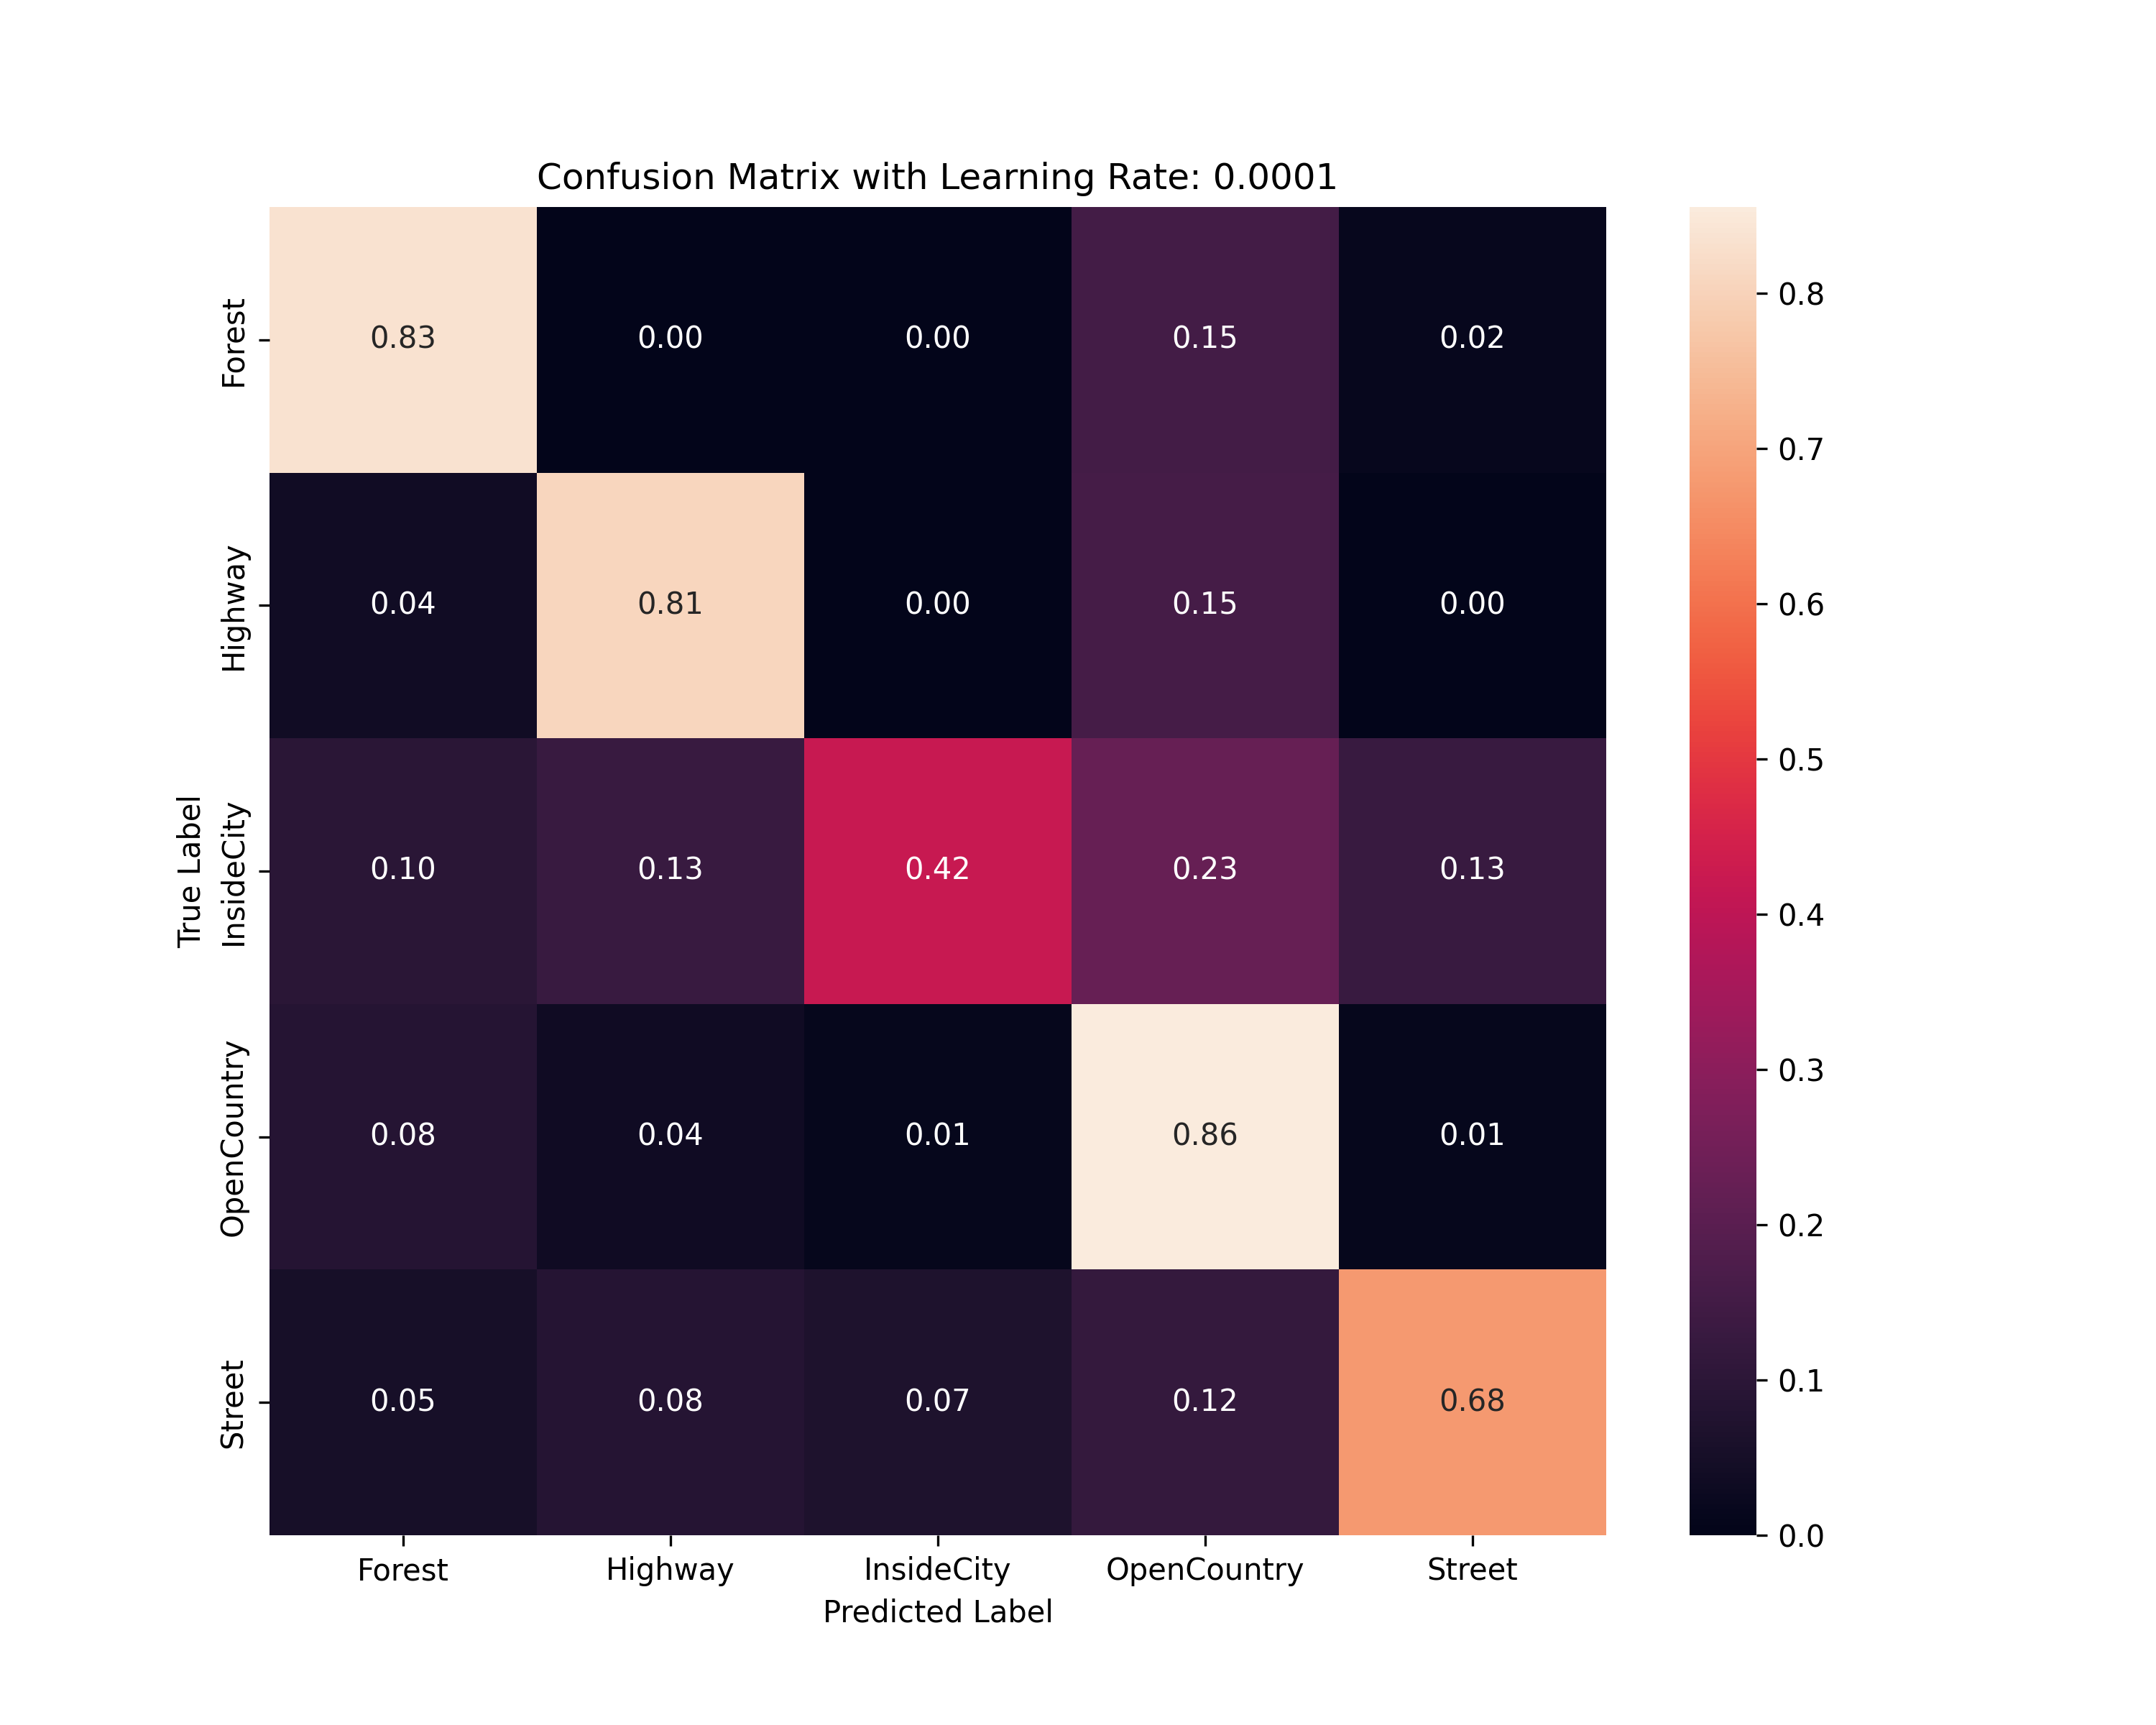
\includegraphics[width=6cm]{confusion_matrix_model_ada_delta_test_0.0001.png} }}%
    \caption{Confusion Matrix for Generalised Delta Rule on training and test dataset}%
    \label{fig:2}%
\end{figure}

\begin{figure}[H]
    \centering
    \subfloat[\centering Training Data]{{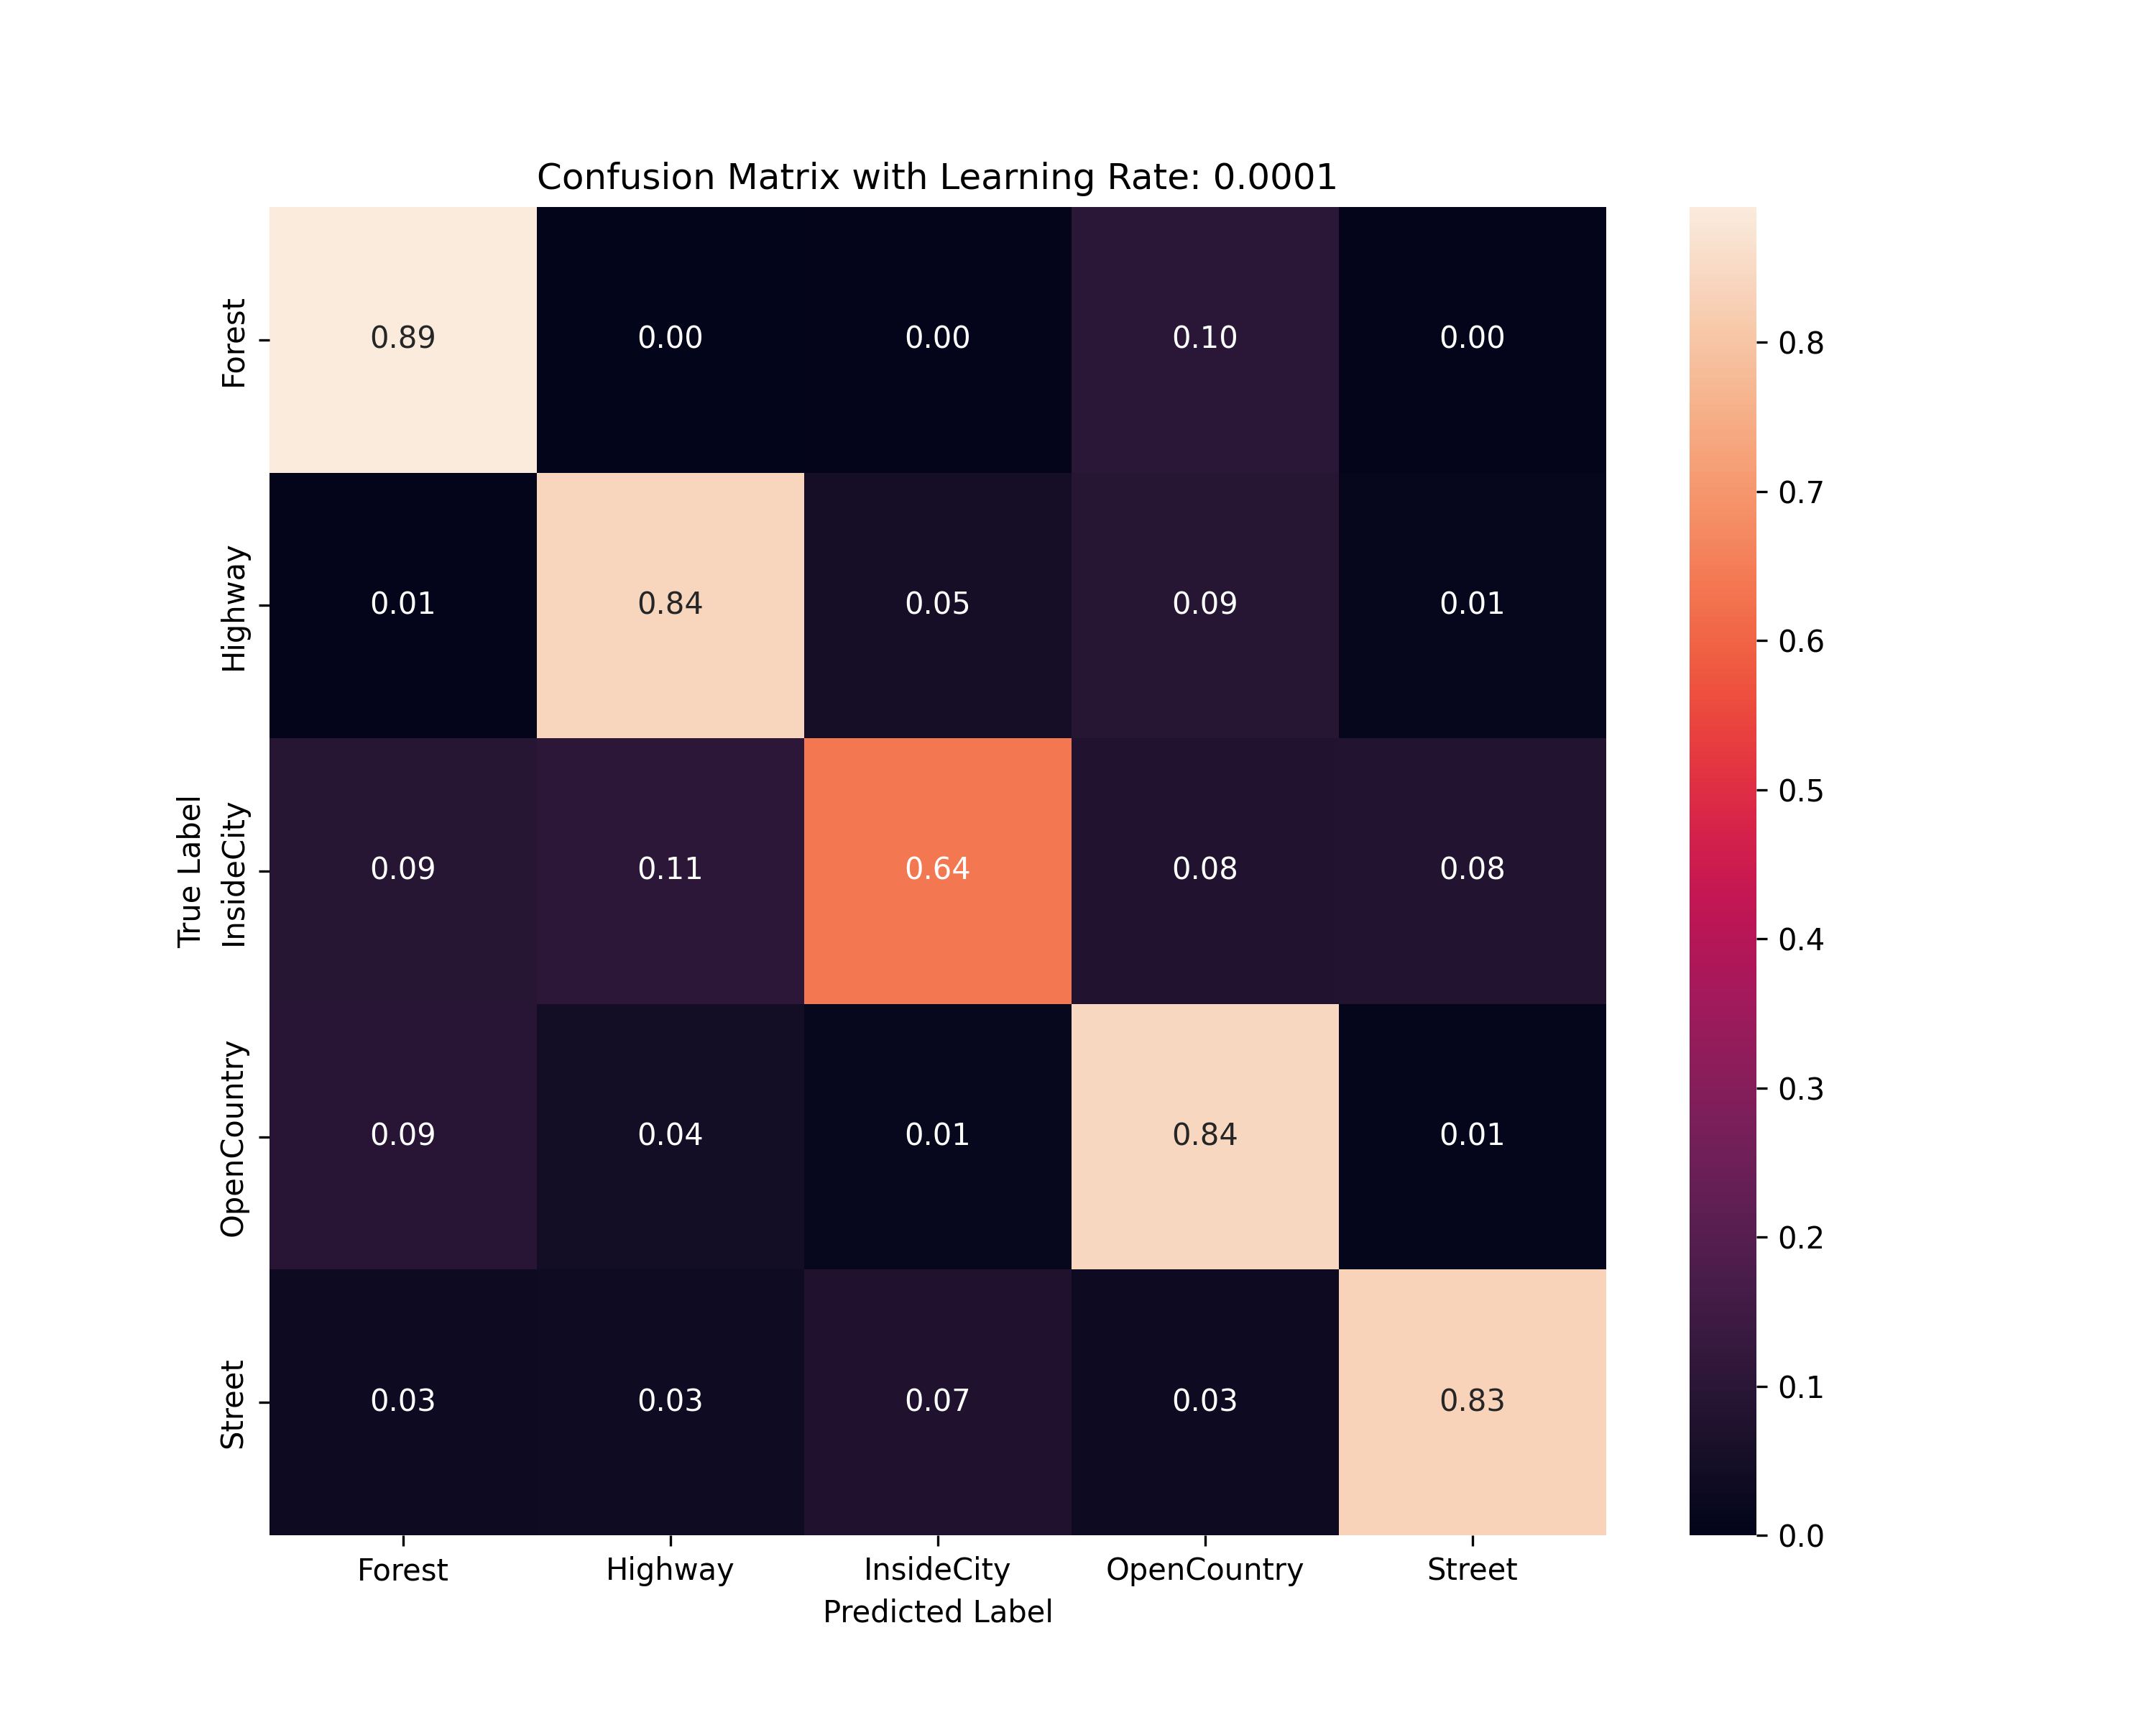
\includegraphics[width=6.5cm]{confusion_matrix_model_adam_train_0.0001.png} }}%
    \qquad
    \subfloat[\centering Test Data]{{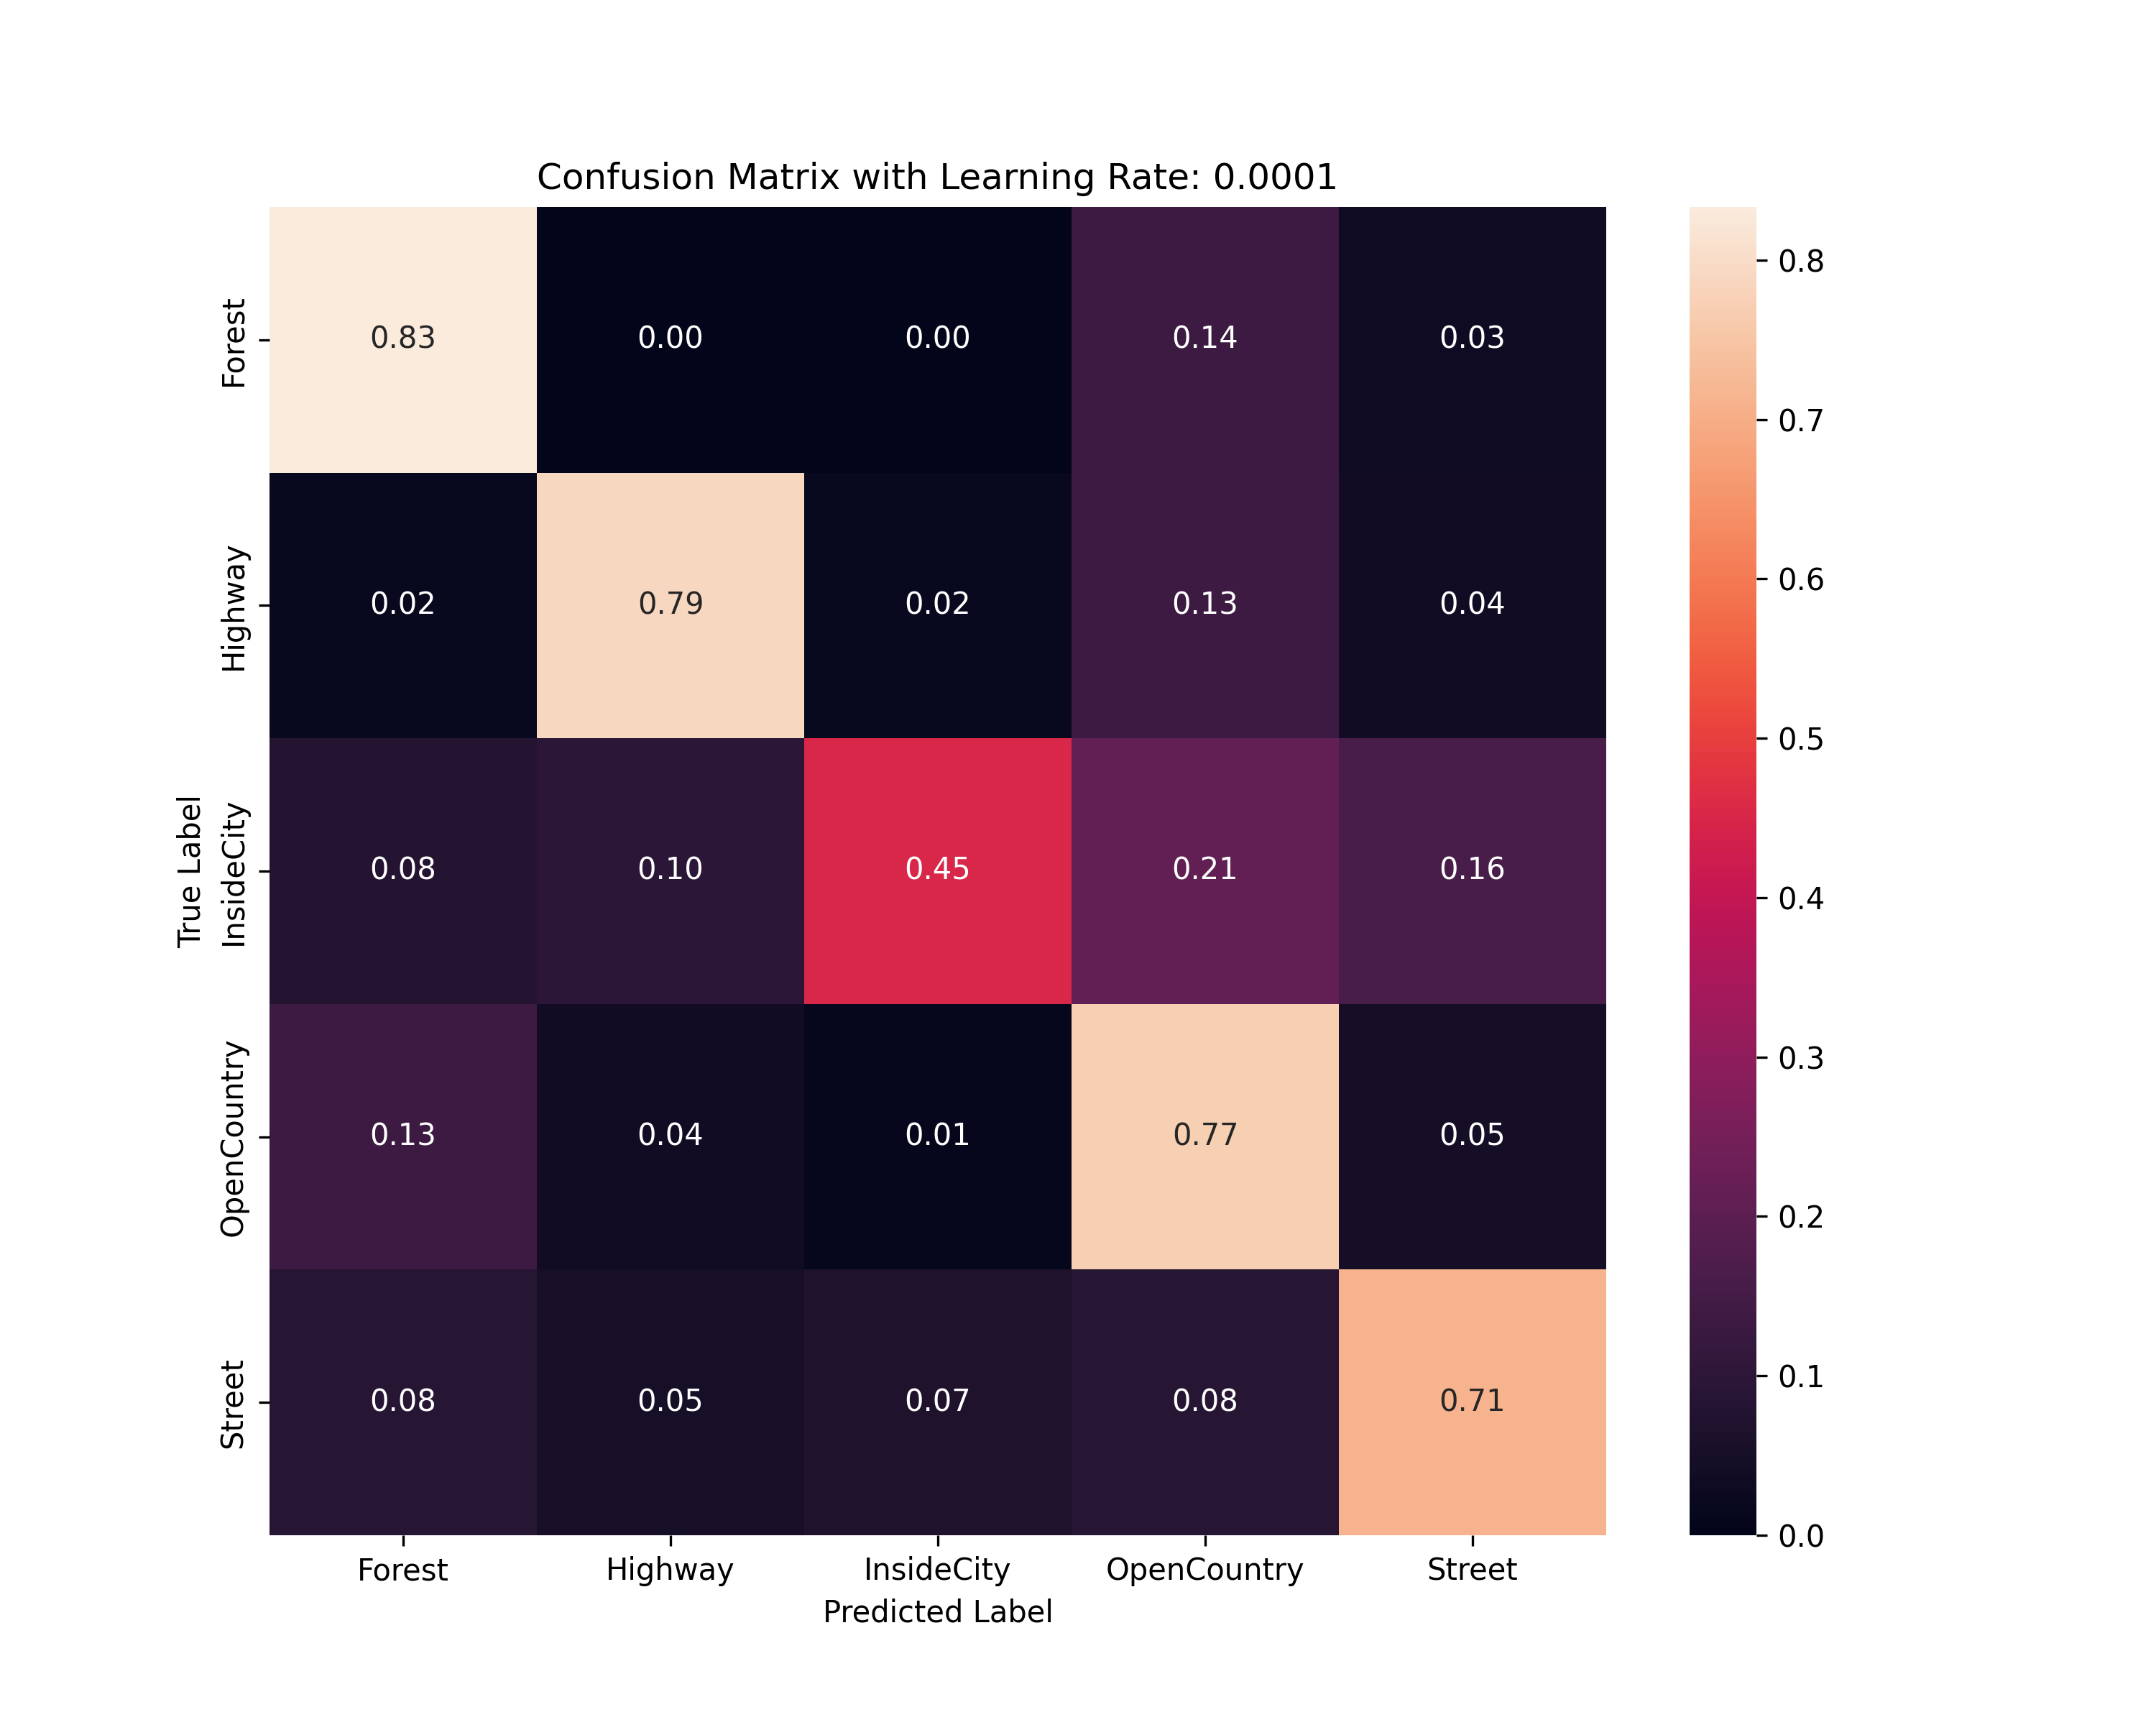
\includegraphics[width=6.5cm]{confusion_matrix_model_adam_test_0.0001.png} }}%
    \caption{Confusion Matrix for Adam Rule on training and test dataset}%
    \label{fig:3}%
\end{figure}

Using our most optimal hyperparameters, we plot the training loss and validation loss variation for different weight update rules.

\begin{figure}%
    \centering
    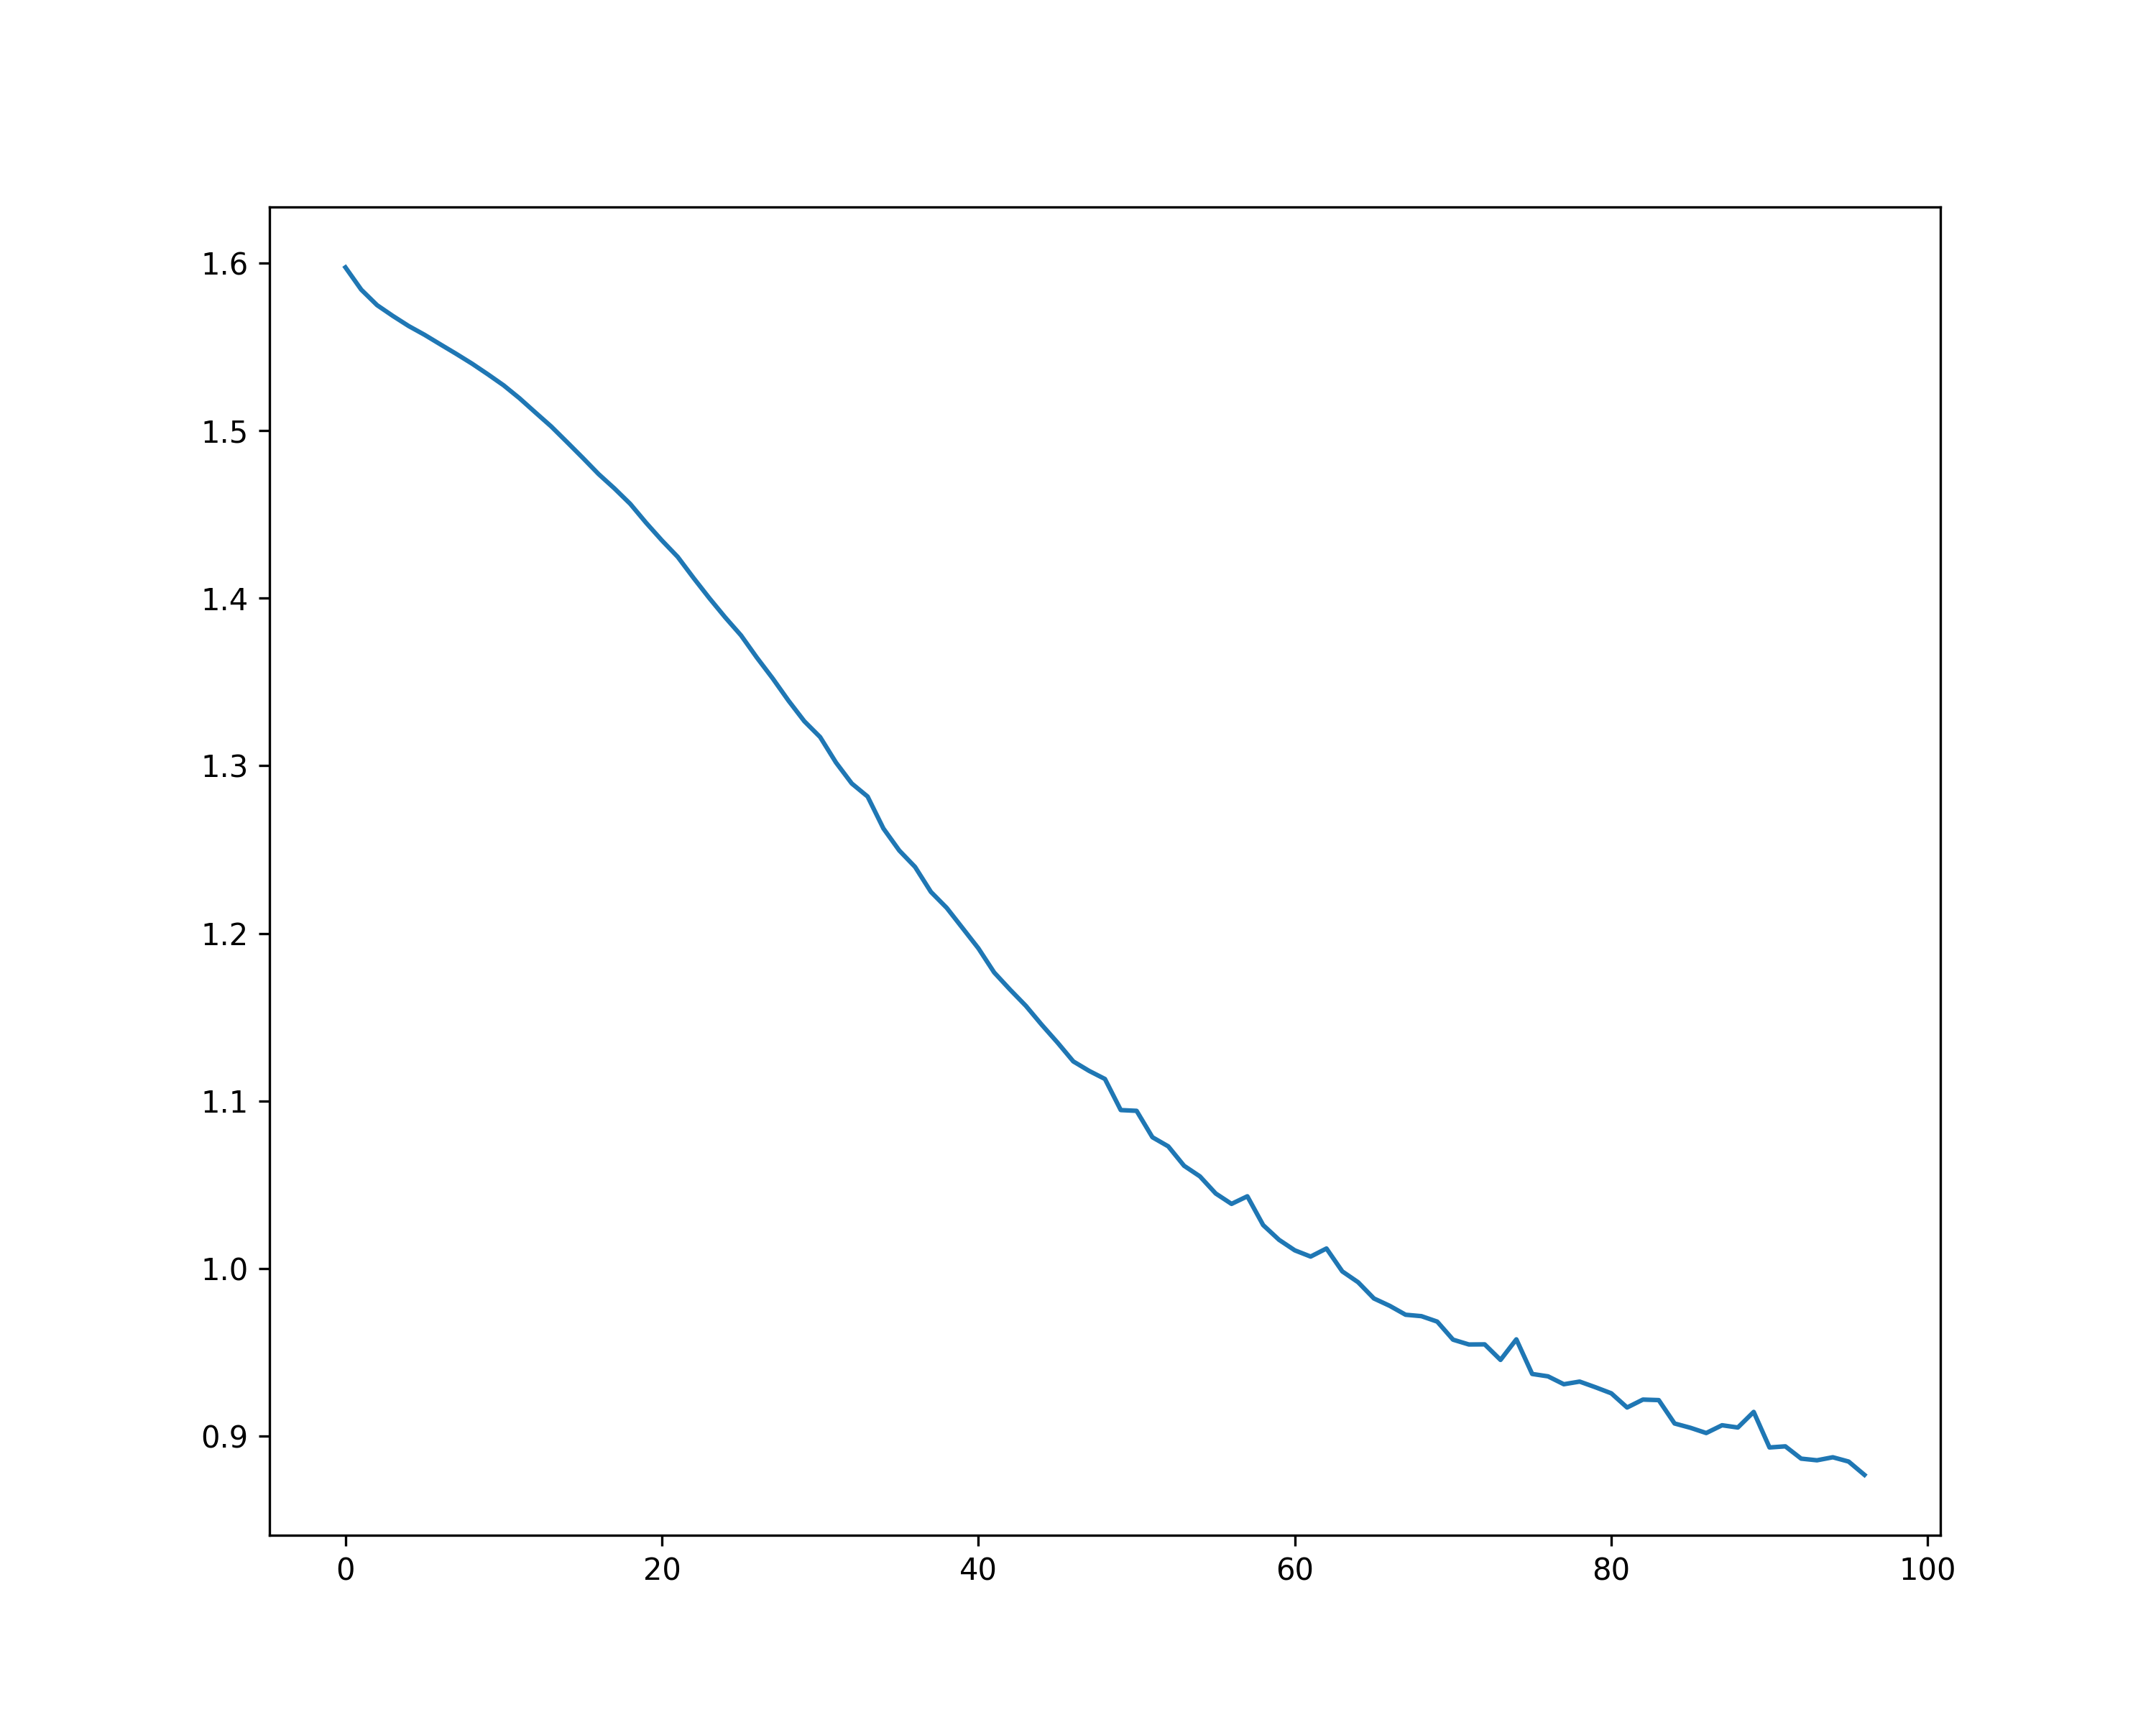
\includegraphics[scale=0.4]{delta_training_loss_0.0001.png}%
    \caption{Training loss vs number of epochs for delta rule}%
    \label{fig:15}%
\end{figure}


\begin{figure}%
    \centering
    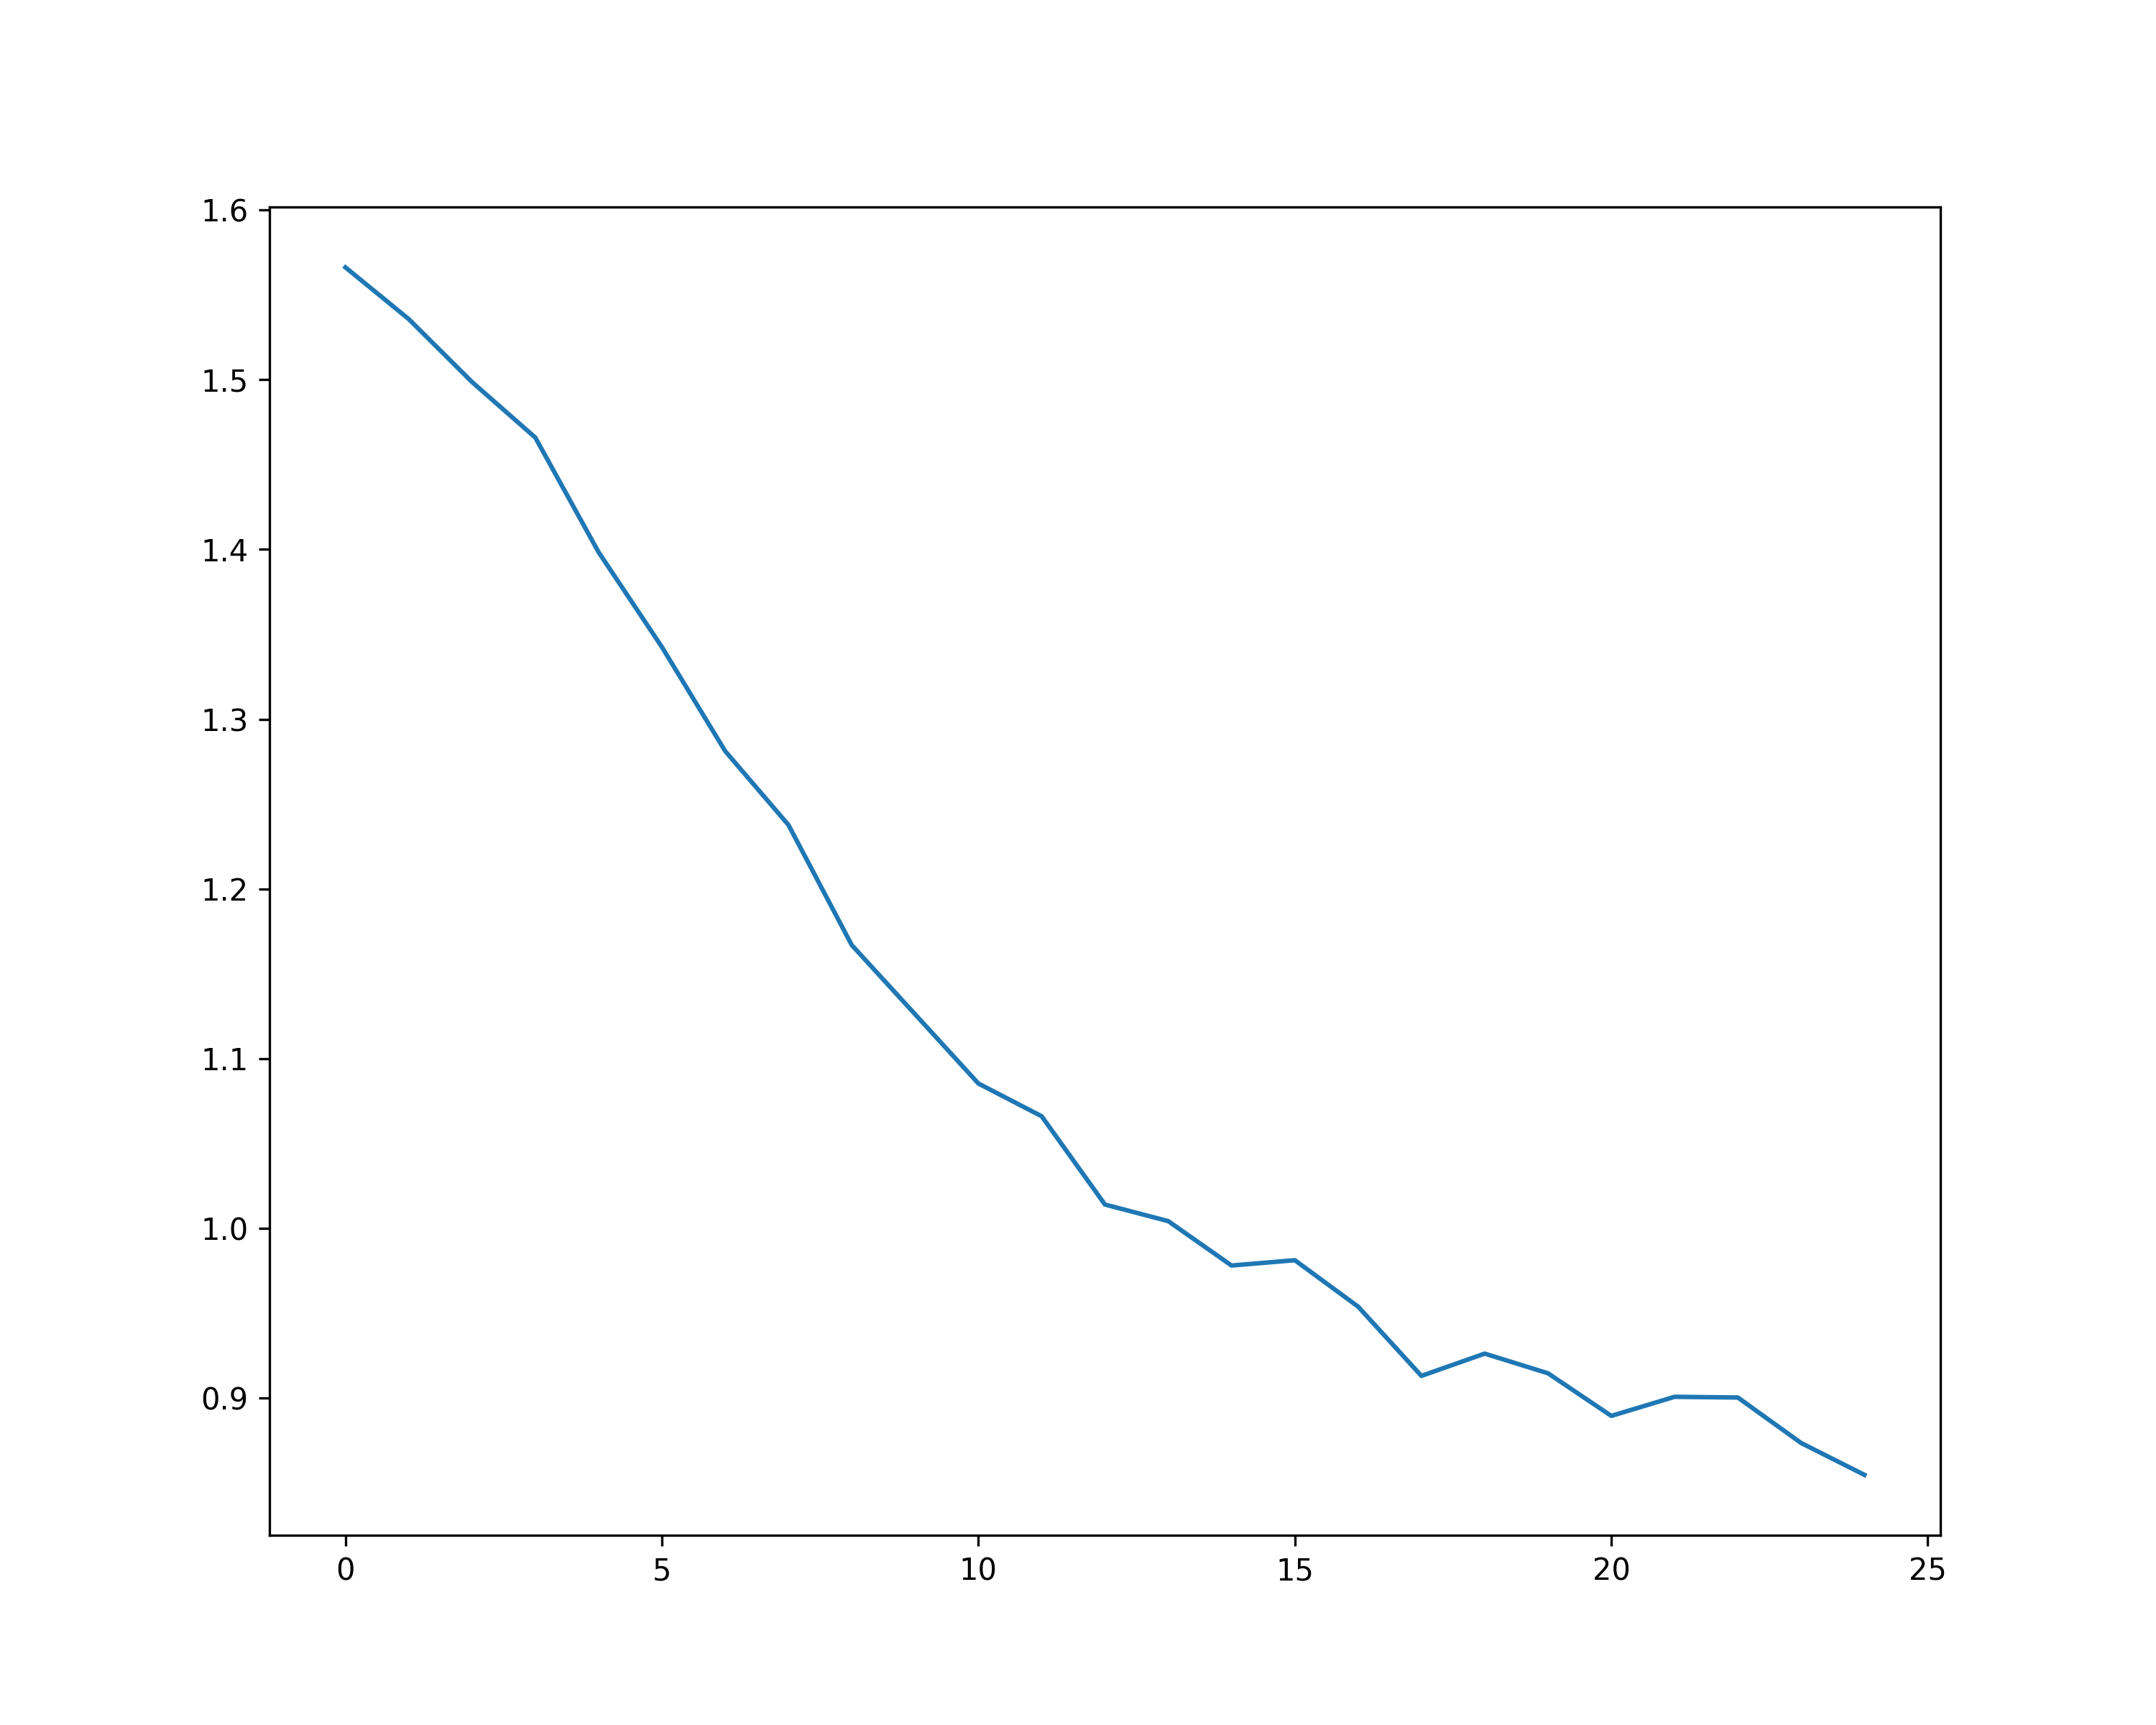
\includegraphics[scale=0.4]{gen_delta_training_loss_0.0001.png}%
    \caption{Training loss vs number of epochs for generalised delta rule}%
    \label{fig:16}%
\end{figure}

\begin{figure}%
    \centering
    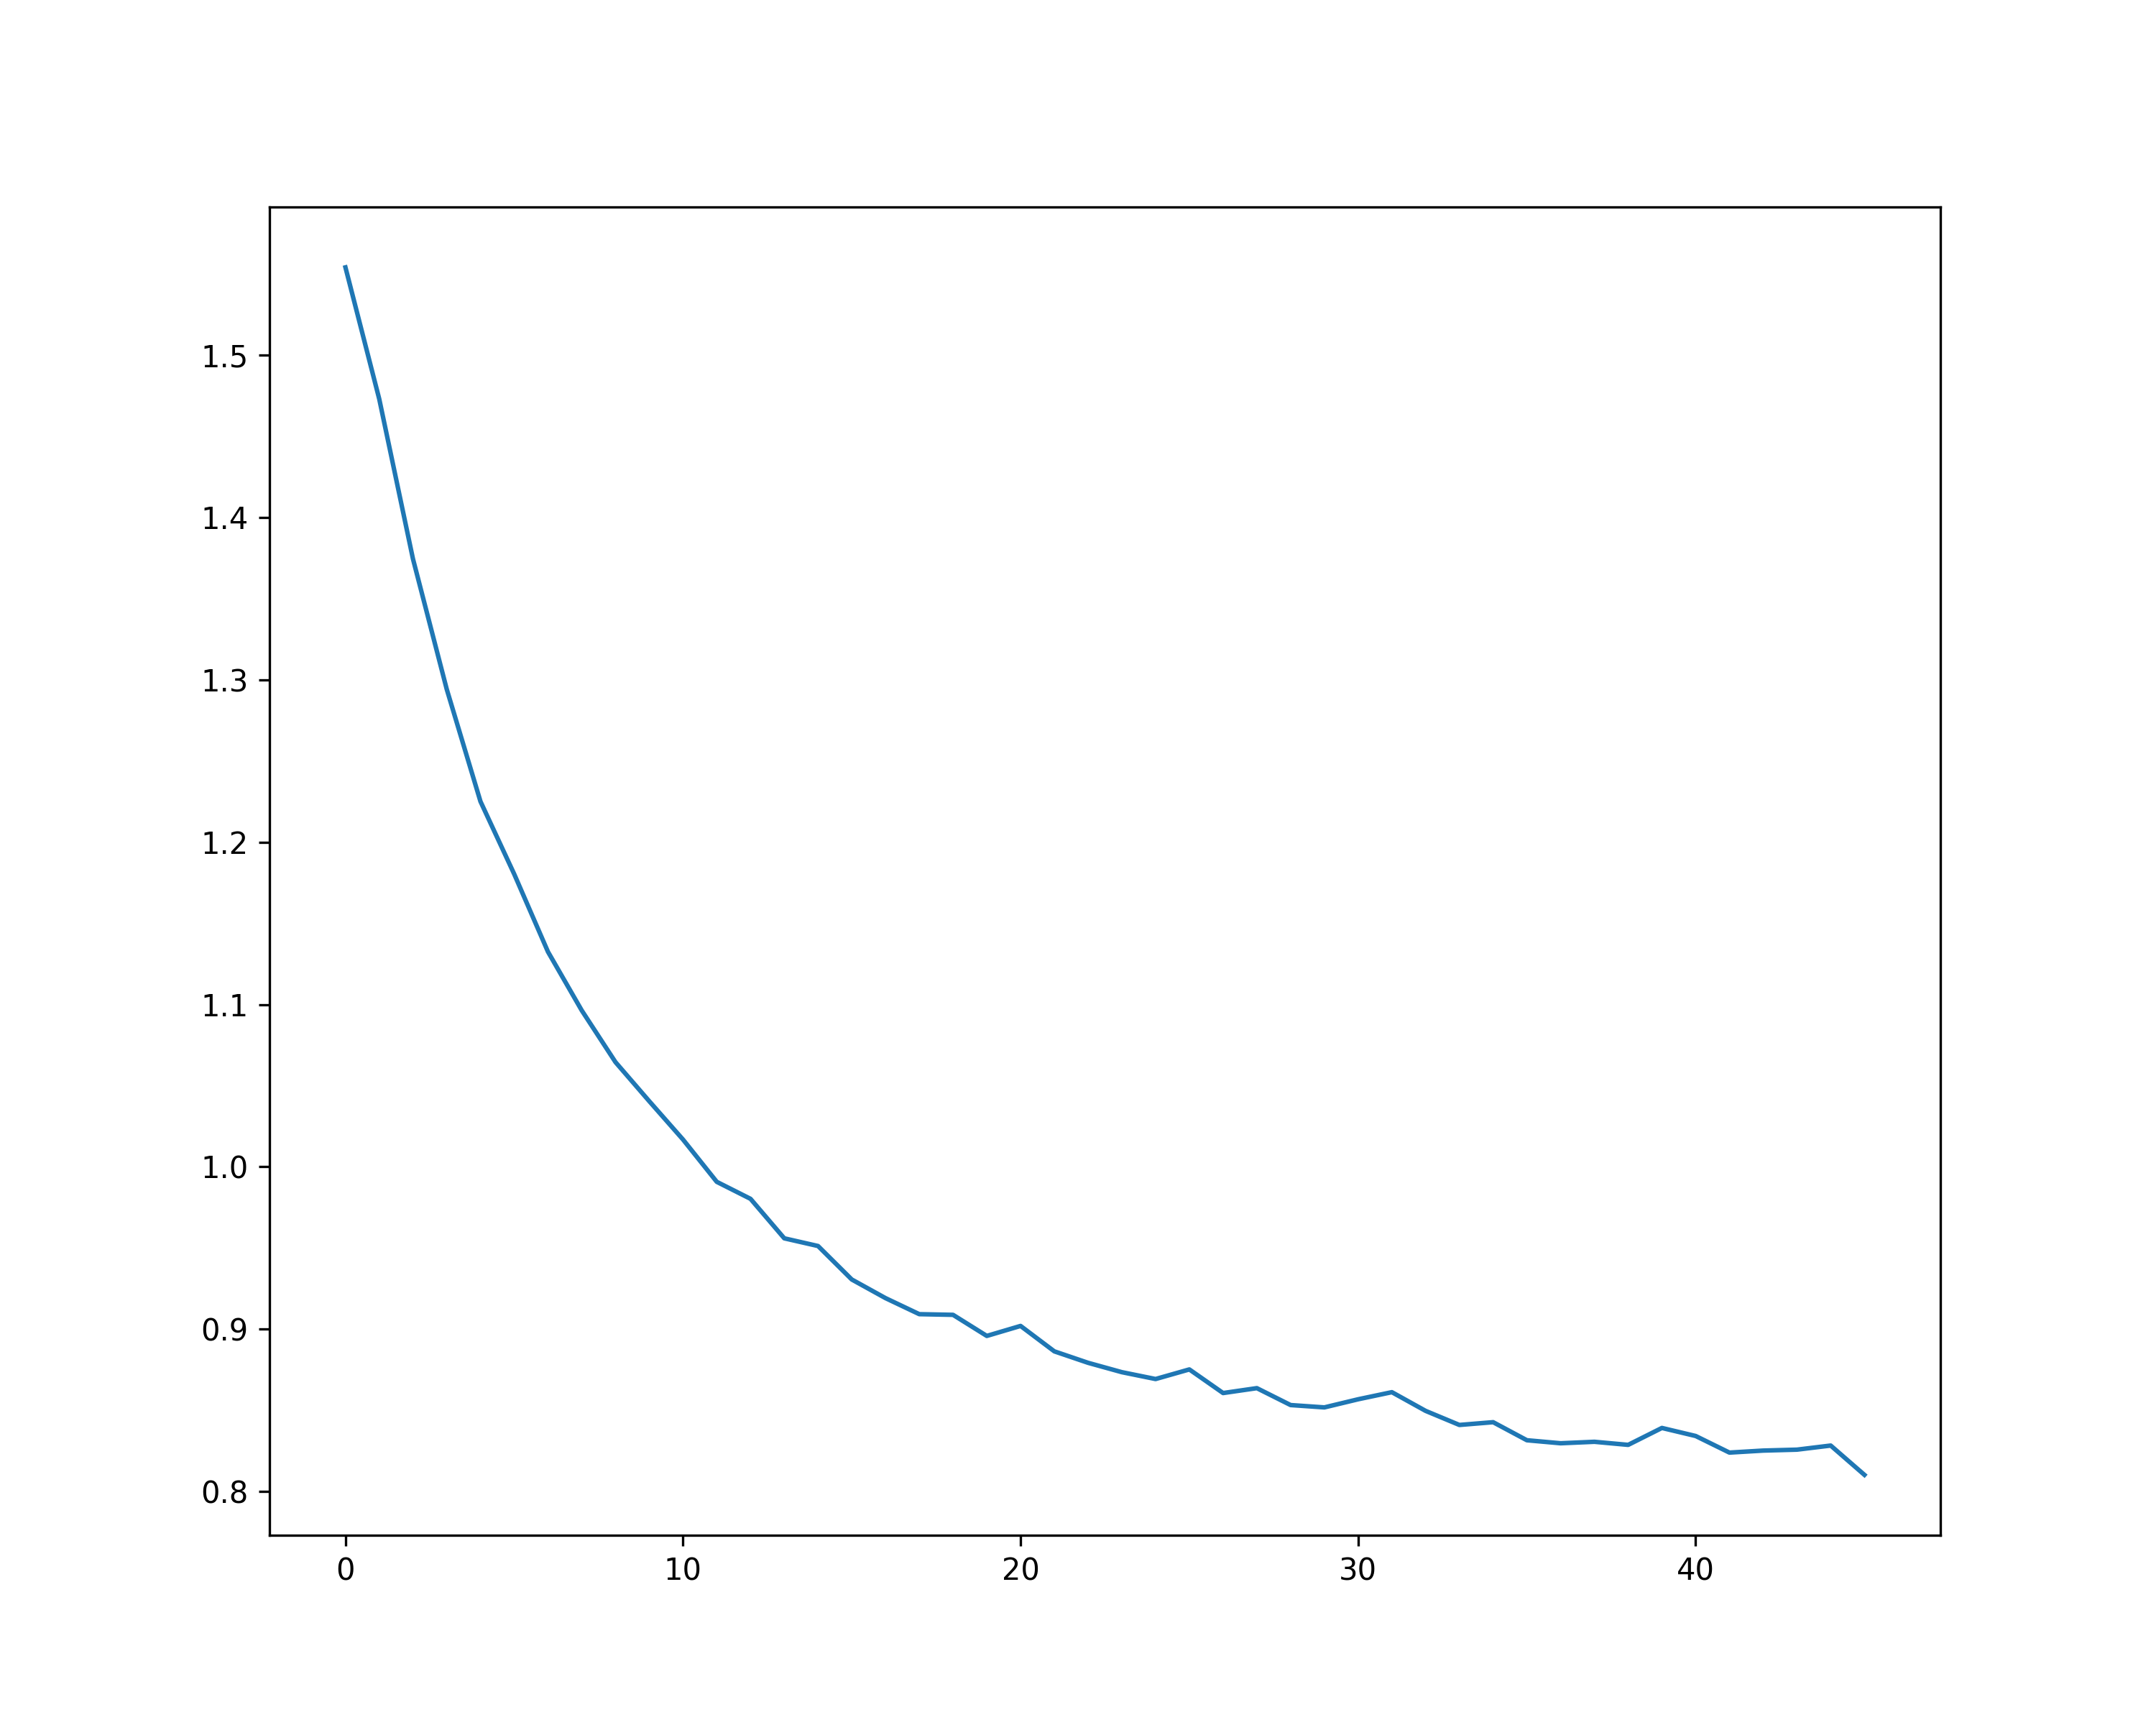
\includegraphics[scale=0.4]{ada_training_loss_0.0001.png}%
    \caption{Training loss vs number of epochs for Adam rule}%
    \label{fig:17}%
\end{figure}


\subsubsection{Number of Epochs taken for different weight update rules}

The epochs taken for convergence for different weight update rules are given in Table 1

\begin{table}[H]
    \centering
\begin{tabular}{l*{3}{c}}
    \toprule
    & \multicolumn{3}{c}{Weight update rule} \\
    \cmidrule(lr){2-4}
    Hyperparameters & Delta & Generalised Delta & Adam \\
    \cmidrule(lr){1-1}
    \cmidrule(lr){2-4}
    (64,64,$1e^{-4}$,0.8) & 116 & 35 & \textbf{22} \\
    (32,32,$1e^{-5}$,0.9) & 500 & 261 & \textbf{88} \\
    (16,16,$1e^{-3}$,0.8) & 11 & 6 & \textbf{2} \\
    \bottomrule
    \label{table1}

    \end{tabular}
    \caption{Comparison of number of epochs taken for different weight update rules. The format of hyperparameters is (number of neurons in hidden layer 1,number of neurons in hidden layer 2,learning rate,momentum (for generalised delta and adam))}
\end{table}

\subsection{Observations}

\begin{itemize}
    \item We observe that Adam converges faster than weight update rules such as delta rule and it is only slightly better than generalized delta rule.
    \item One interesting observation that we make is that even though Adam converges faster, delta generalizes better than Adam and thus results in slightly improved final performance.
    \item Also, the validation loss of delta and generalized delta rule is more stable compared to Adam rule.
    \item The reason why Adam converges faster is that it adaptively selects a separate learning rate for each parameter. 
    Parameters that would ordinarily receive smaller or less frequent updates receive larger updates with Adam
    \item In the confusion matrix, we observe that the model gets confused between classes such as insidecity and street which is to be expected as both classes are
    visually similar
    \item When the learning rate is lesser than $1e^{-4}$, the time taken for convergence (especially for delta rule) is much longer.
    \item When the value of momentum is less such as 0.2-0.5, time taken for generalised delta and delta is quite similar.
    \item Also, overfitting is very much prelavent as number of neurons increase in the hidden layer. To mitigate that, we use early stopping rule. x`'

\end{itemize}

\end{document}
